\documentclass[../main.tex]{subfiles}

\begin{document}


\begin{wrapfigure}[23]{r}{0.6\textwidth}
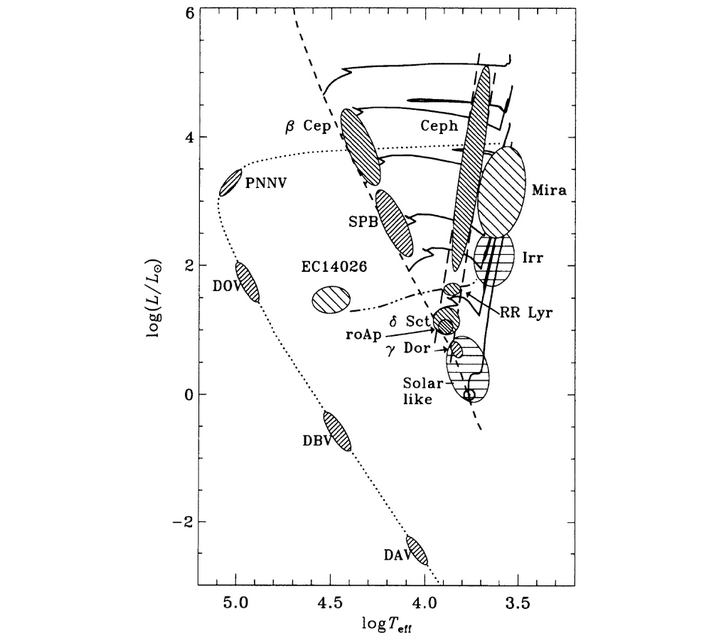
\includegraphics[width=0.65\textwidth,keepaspectratio]{HRpulsating} \label{fig:HRp}
\caption{Zone del diagramma di \hr{} in cui sono previsti comportamenti oscillatori. Da \cite{chr97lecture}.}
\end{wrapfigure}

\vfill

La struttura stellare \'e determinata da massa e composizione chimica iniziale della stella sulla base delle condizioni di equilibrio idrostatico e termico locale.

I modelli stellari contengo dei parametri per descrivere i fenomeni fisici per cui non esiste una teoria completa: i parametri vengono scelti in maniera da riprodurre pi\'u accuratamente possibile la posizione della stella nel diagramma di \hr{}, definito da luminosit\'a e temperatura efficace.

%Un modello stellare deve riprodurre la posizione di una stella nel diagramma entro le incertezze sulle osservabili sperimentali disponibili: luminosi\'a, massa, raggio, spettro della luce emessa dalla superficie (temperatura efficace, composizione chimica superficiale, accelerazione di gravit\'a) ed et\'a.

\'E possibile che parte dell'energia interna di una stella alimenti un comportamento oscillatorio attorno alla configurazione di equilibrio: le frequenze dei modi normali sono le osservabili sperimentali che contengono informazioni dirette sull'interno stellare, oltre al flusso di neutrini prodotti nelle reazioni nucleari.

 Nei capitoli successivi descrivo la configurazione di equilibrio del Sole e le incertezze nella descrizione fisica del modelo solare standard (MSS).


{\let\clearpage\relax\let\cleardoublepage\relax
\chapter{Strutture autogravitanti in equilibrio}
}

\section{Condizione di equilibrio idrostatico.}

Suppongo che la pressione del campo magnetico sia molto minore della pressione del gas nell'interno solare e che la correzione dovuta alla rotazione sia piccola, ci\'o \'e suffragato dalle misure del campo magnetico superficiale e dalla piccola deviazione dalla forma sferica.

%tensore pressione$\to$hydrostatic pressure

La distribuzione di massa del Sole \'e determinata dall'equilibrio tra la forza di attrazione gravitazionale e il gradiente della pressione del gas. Considero una distribuzione di massa sferica con densit\'a $\rho(r,t)$, la variazione della massa presente entro il raggio $r$ \'e descritta da

\begin{equation}
dm=4\pi r^2\rho \,dr-4\pi r^2\rho v\,dt\label{eq:massvar}
\end{equation}

e $v(r,t)$ \'e il campo di velocit\'a della distribuzione di massa a distanza r dal centro e tempo $t$,

%Eulerian vs Lagrangian description

per una configurazione di equilibrio statico quindi

\begin{equation}
dm=4\pi r^2\rho \,dr\label{eq:massaguscio}
\end{equation}

Differenziando \eqref{eq:massvar} rispetto alle variabili euleriane $r$ e $t$ ricavo l'equazione di continuit\'a

\begin{align}
&\PDy{t}{\rho}=-\frac{1}{r^2}\PDof{r}(\rho r^2 v)&\intertext{che esprime la conservazione della massa per simmetria sferica, in generale}\nonumber\\
&\PDy{t}{\rho}+\nabla\cdot(\rho\vec{v})=0\label{eq:continuityeq}
\end{align}

La condizione di equilibrio idrostatico $\ddvec{r}=0$ implica, per la conservazione della quantit\'a di moto

\begin{align}
&\rho\TDy{t}{\vec{v}}=-\nabla P+\rho\vec{f}\label{eq:motion}&\intertext{da cui segue}\nonumber\\
&\nabla P=\rho \vec{f}\label{eq:idrosta}
\end{align}

Nel caso di una stella la forma della forza per unit\'a di massa f \'e determinata dall'attrazione gravitazionale

\begin{equation}
g=\frac{Gm(r)}{r^2}\label{eq:gravitya}
\end{equation}
diretta verso il centro di massa.

Definendo il potenziale gravitazionale $\Phi$, soluzione dell'equazione di Poisson 
\begin{equation}
\nabla^2\Phi=4\pi G\rho\label{eq:poisson}
\end{equation}
risulta:
\begin{equation}
\vec{g}=-\PDy{r}{\Phi}=-\frac{Gm(r)}{r^2}\hat{r}
\end{equation}

La condizione di equilibrio idrostatico diventa:
\begin{equation}
\TDy{r}{P}=-\frac{Gm(r)\rho(r)}{r^2}\label{eq:fidroequilibrio}
\end{equation}



Considero il contributo alla pressione degli ioni, elettroni e fotoni, $P=P_I+P_e+P_R$. Il gas solare \'e approssimabile come un gas perfetto essendo composto in gran parte da \chem{H} e \chem{^4He} completamente ionizzati con distanza interionica $a_0$ molto maggiore delle dimensioni nucleari
\begin{align}
&a_0=(\frac{3}{4\pi}\sum_{I}n_I)\expy{-\frac{1}{3}}\gg r_N\label{eq:interionicdistance}\\
&P_I=\rho \gasconstant{} T(X+\frac{Y}{4}+\frac{Z}{\exv{A_Z}})\shortintertext{dove ho usato il peso molecolare medio per i soli ioni $\mu_0$,}\nonumber\\
&P_R=\frac{a}{3}T^4\intertext{definisco il parametro $\beta$}\nonumber\\
&P_R=(1-\beta)P
\end{align}

Il peso molecolare medio, definito come massa media in amu per particella libera \'e

\begin{equation}
\mu=\frac{1}{\bar{n}_HX+\bar{n}_{He}Y+\bar{n}_{Z}Z}\label{eq:meanmw},\ \mu_0=\frac{1}{X+\midfrac{Y}{4}+\midfrac{Z}{\bar{A}}}
\end{equation}

con $\bar{n}_i=\frac{1+f_i}{A_i}$ numero medio di particelle libere per unit\'a di massa atomica dovute alla specie i di peso atomico $A_i$ con $f_i$ numero medio di elettroni liberati da specie i.

Trascurando la degenerazione degli elettroni

\begin{equation}
P_G=P_I+P_e=\frac{\rho}{\mu}\gasconstant{}T
\end{equation}

\subsection{Tempo di evoluzione dinamico.}

Scrivo l'equazione del moto per la massa $dm$ racchiusa da un guscio sferico di raggio r:
\begin{align}
&\frac{dm}{4\pi r^2}\PtwoDy{t}{r}=f_P+f_g\shortintertext{dove il primo termine sulla destra \'e il contributo dovuto alla differenza di pressione fra i due bordi del guscio, mentre il secondo \'e il contributo della forza di gravit\'a. Esplicitando gli addendi sulla destra e differenziando rispetto a $m$ si ha:}\nonumber\\
&\frac{1}{4\pi r^2}\PtwoDy{t}{r}=-\PDy{m}{P}-\frac{Gm}{4\pi r^4}\label{eq:motionshell}
\end{align}

Per giustificare l'ipotesi di equilibrio idrostatico stimo i tempi caratteristici di evoluzione della struttura solare nel caso la forza dovuta alla pressione o la forza di gravit\'a non fossero bilanciate, approssimando il valore caratteristico della derivata di due variabili con il rapporto del loro valore caratteristico:
\begin{align}
&\tau_{ff}\approx\sqrt{\frac{\rsun{}}{g}}\shortintertext{tempo caratteristico di una distribuzione sferica di materia in caduta libera cio\'e considerando solo il secondo termine in \eqref{eq:motionshell},}\nonumber\\
&\tau_{esp}\approx \rsun{}\sqrt{\frac{\rho}{P}}\shortintertext{tempo caratteristico di espansione dovuta al termine di pressione esclusivamente.}\nonumber
\end{align}

Per i valori
\begin{align}
&G\msun=\num{132712440018+-8}\SI{e9}{\cubic\meter\per\square\second}\\
&\rsun{}=\SI{6.9626+-0.0007}{\meter}
\end{align}
ottengo valori di circa $27$ min.: quindi la costanza delle caratteristiche solari su tempi molto maggiori giustifica l'ipotesi di equilibrio idrostatico, quindi  riscrivo il tempo scala di evoluzione dinamica come

\begin{equation}
\tau_{idro}^{\odot}= \sqrt{\frac{R^3}{GM}}\approx\frac{1}{2}(G\overline{\rho})\expy{-\frac{1}{2}}\approx\SI{27}{\minute}
\end{equation}


\section{Conservazione dell'energia.}

Il collasso di una nube di gas interstellare \'e un processo complesso. Quando si raggiunge una configurazione abbastanza densa, tale che il cammino libero medio degli atomi e dei fotoni sia breve, si raggiunge rapidamente l'equilibrio idrostatico e termico locale. Il processo di collasso gravitazionale continua fino a che l'energia prodotta dalle reazioni nucleari bilancia l'energia irradiata.

\subsection{Teorema del viriale.}

Il teorema del viriale esprime una propriet\'a statistica di particelle interagenti: si trova una relazione tra energia interna, dovuta al moto traslazionale degli atomi, ed energia potenziale gravitazionale.

L'energia potenziale gravitazionale della stella \'e
\begin{equation}
\Omega=-\int_0^M\frac{Gm(r)}{r}\,dm\label{eq:energiapg}
\end{equation}

mentre l'energia interna \'e costituita dalla somma delle energie traslazionali delle particelle pesate secondo la distribuzione di equilibrio di Maxwell-Boltzmann

\begin{equation}
E_i=\int_0^Mu\,dm=\int_M\frac{1}{\rho}\int n(\vec{p})\frac{p^2}{2m}\,d\vec{p}\,dm=\frac{3}{2}\int_M\frac{P}{\rho}\,dm
\end{equation}

dove $n(\vec{p})$ \'e il numero di particelle per unit\'a di volume con impulso in $[\vec{p},\vec{p}+d\vec{p}]$ e u \'e l'energia interna per unit\'a di massa.

Il teorema del viriale dimostra che

\begin{equation}
\frac{1}{2}\TtwoDy{t}{I}=2K+\Omega
\end{equation}

con K energia cinetica e $I=\int r^2\,dm$, implica, dato che all'equilibrio $\frac{1}{2}\TtwoDy{t}{I}=0$

\begin{equation}
0=\int_M\frac{3P}{\rho}\,dm(r)+\Omega
\end{equation}


Detta $W=E_i+\Omega$ l'energia totale della stella, 
\begin{equation}
\Omega=-2E_i\label{eq:virialegpm}
\end{equation}

e dalla conservazione dell'energia $\TDy{t}{W}+L=0$ segue che durante la fase di collasso prima dell'inizio della sequenza principale met\'a dell'energia gravitazionale viene spesa per aumentare l'energia interna e met\'a in luminosit\'a:

\begin{equation}
L=-\frac{1}{2}\dot{\Omega}=\dot{E}_i
\end{equation}


Il tempo caratteristico che regola il collasso gravitazionale di una massa gassosa in equilibrio idrostatico \'e il tempo di Kelvin-Helmholtz
\begin{equation}
\tkh{}=\frac{\Omega}{L}\approx\frac{GM^2}{2RL}
\end{equation}
sostituendo i valori solari con $\lsun{}=\SI{3.846e33}{\erg\per\second}$ si ha $\tkh{}\approx\SI{1.6e7}{\year}$.


\subsection{Conservazione dell'energia interna}

La prima legge della termodinamica esprime la conservazione dell'energia interna, ovvero mette in relazione il flusso di calore $dq$ per unit\'a di massa in un elemento di gas nell'intervallo di tempo $dt$ con la variazione di energia interna per unit\'a di massa $du$ e di volume specifico $dV$:
\begin{equation}
\TDy{t}{q}=\TDy{t}{u}+P\TDof{t}(\frac{1}{\rho})=0=\TDy{t}{u}+P\TDy{t}{V}\label{eq:prima}
\end{equation}

che posso riscrivere come

\begin{align}
&\TDy{t}{\ln{T}}=\frac{\Gamma_2-1}{\Gamma_2}\TDy{t}{\ln{P}}+\frac{\TDy{t}{q}}{c_PT}\label{eq:primatemp}\\
&\TDy{t}{\ln{P}}=\Gamma_1\TDy{t}{\ln{\rho}}+\frac{\rho(\Gamma_3-1)}{P}\TDy{t}{q}\label{eq:primapres}
\end{align}

dove ho introdotto gli esponenti adiabatici $\Gamma_i$

\begin{equation}
\Gamma_1=\Dcvar{\TDly{\rho}{P}}{Ad}, \ \Gamma_3-1=\Dcvar{\TDly{\rho}{T}}{Ad},\ \frac{\Gamma_2-1}{\Gamma_2}=\Dcvar{\TDly{P}{T}}{Ad}
\end{equation}

L'energia interna per unit\'a di massa \'e approssimabile con quella di un gas perfetto: 

\begin{equation}
u(T,P)=\frac{3\gasconstant{}T}{2\mu}
\end{equation}

%Il contributo delle modificazioni chimiche aggiungo al lato di destra di \eqref{eq:prima} il termine contenente il potenziale chimico $-\mu_idN_i$ con $\mu_i=\Dcvar{\PDy{N_i}{u}}{S,V}$ all'equilibrio \'e trascurabile.
%Vedi: chemical mixing, equilibrium slowness (partial ionization region, nuclear burning) mass action law: $\sum n_i\mu_i=0$??, minimizzazione energia libera.

Scrivo il bilancio di calore per un elemento di massa unitaria di gas:

\begin{equation}
\TDy{t}{q}=\epsilon-\frac{1}{\rho}\nabla\cdot\vec{F}\label{eq:heatgl}
\end{equation}
dove $\epsilon$ \'e l'energia prodotta per unit\'a di tempo e massa dalle reazioni nucleari e $\vec{F}$ \'e il flusso di energia verso l'esterno che in situazioni di stabilit\'a dinamica \'e dovuto alla diffusione di fotoni dalla zona pi\'u calda verso la superficie; sostituendo in \eqref{eq:prima} si ha

\begin{equation}
\TDy{r}{L}=4\pi r^2[\rho\epsilon-\rho\TDof{t}u+\frac{P}{\rho}\TDy{t}{\rho}]\label{eq:fenergyconservation}
\end{equation}

Tengo conto dell'energia generata sotto forma di neutrini, che, alle densit\'a tipiche dell'interno solare, hanno interazioni trascurabili con la materia e quindi non danno luogo a un flusso di calore nel sistema, aggiungendo un termine negativo $-\epsilon_{\nu}$ tale che $L_{\nu}=\int_0^M\epsilon_{\nu}\,dm$.

Nel caso stazionario

\begin{equation}
\TDy{t}{q}=0\ \Rightarrow\ dL=4\pi r^2\rho\epsilon\,dr
\end{equation}
e i processi nucleari che avvengono nella parte centrale forniscono il calore per bilanciare il flusso di energia uscente, in particolare le reazioni delle catene $\Pproton\Pproton$ contribuiscono per il $99.9\%$ all'energia generata da reazioni nucleari nel Sole.

Stimo il tempo trascorso da una stella di massa solare in sequenza principale considerando il tempo necessario per la massa di idrogeno nel core di fusione (le temperature necessarie perch\'e il rate di reazione sia apprezzabile si raggiungono nella regione pi\'u interna che costituisce una frazione $f$ pari al $15\%$ della massa solare) a trasformarsi in elio:

\begin{equation}
\tau_n\approx\frac{E_n}{L}=\frac{fX\msun Q}{\lsun}\approx\SI{e+10}{\year},\ Q=\SI{6.3e18}{\erg\per\gram}
\end{equation}


{
\let\clearpage\relax\let\cleardoublepage\relax
\chapter{Costruzione del modello solare}
}

Per quanto riguarda il Sole \'e possibile determinare sperimentalmente il prodotto $G\msun$, la distanza, la luminosit\'a, la composizione chimica al livello della fotosfera, ad eccezione del $\cel{He}{4}{}{}$ e altri gas nobili, e il raggio; allo stato delle conoscenze \'e conveniente introdurre un parametro $\alpha$ per descrivere l'efficienza del trasporto convettivo da determinare tramite la calibrazione del modello con le osservazioni, assieme all'abbondanza di $\cel{He}{4}{}{}$.


\section{Equazione di stato e energia interna.}

Gli approcci pi\'u usati per determinare l'equazione di stato e quindi le grandezze termodinamiche del plasma solare sono due. Lo schema chimico considera atomi e molecole, la cui popolazione per stati eccitati e diversi gradi di ionizzazione \'e ottenuto minimizzando l'energia libera; utilizzando questo approccio \'e stata ricavata l'equazione di stato MHD. Lo schema fisico considera nuclei ed elettroni come costituenti fondamentali interagenti tramite potenziale Coulombiano e trova le soluzione dell'equazione di Schr\"oedinger per un problema a molti corpi, questo approccio, usato per ricavare l'equazione di stato OPAL, \'e pi\'u adatto per trattare le regioni interne del Sole.

L'energia libera \'e connessa all'equazione di stato e alle altre grandezze termodinamiche da

\begin{align}
&P(\rho,T)=\frac{1}{\rho^2}\Dcvar{\PDy{\rho}{F}}{T},\ u=-T^2\PDof{T}\left(\frac{F}{T}\right)
\end{align}
 
Elenco alcune correzioni all'equazione dei gas perfetti:

\begin{itemize}

\item Stati elettronici legati e stati di scattering; ionizzazione da pressione.


Nelle regioni di ionizzazione parziale di $\cel{H}{1}{}{}$ e $\cel{He}{4}{}{}$ considero un contributo all'energia interna per unit\'a di massa dell'energia di legame degli elettroni 

%u(T,P)=\frac{3\gasconstant{}T}{2\mu}+\frac{1}{\rho}[n_{H^+}\chi_H+n_{He^+}\chi_{He}+n_{He^{++}}(\chi_{He}+\chi_{He^+})]
\begin{equation}
\frac{1}{\rho}[n_{H^+}\chi_H+n_{He^+}\chi_{He}+n_{He^{++}}(\chi_{He}+\chi_{He^+})]
\end{equation}

con $\chi_x$ energia di ionizzazione dell'atomo $x$ e $n(x^i)$ densit\'a dell'atomo $x$ ionizzato i volte calcolato tramite l'equazione di Saha che tuttavia non tiene conto della ionizzazione da pressione dovuta alle modificazioni dei livelli atomici indotte dalla materia circostante.

Inoltre si hanno correzioni per gli stati di scattering.

\item Degenerazione degli elettroni.

Il contributo degli elettroni, detta $n_e$ la densit\'a numerica, $\psi(P,T)$ il parametro di degenerazione, tale che per $\psi\to-\infty$ si abbia la distribuzione di Boltzmann e per $\psi\to+\infty$ completa degenerazione, e $u_k$ energia cinetica dell'elettrone, \'e determinato da
\begin{align}
&\rho N_A\frac{1+X}{2}=\intzi{}\frac{8\pi p^2\,dp}{h^3(\exp{\frac{u_k}{KT}-\psi}+1)},\ \beta P-\rho\gasconstant{}(X+\frac{Y}{4}+\frac{Z}{\exv{A_Z}})=\frac{1}{3}\intzi{}pn_e\TDy{p}{u_k}\,dp\shortintertext{dove ho introdotto il peso atomico medio per elettrone libero (ionizzato) $\mu_e$ con}\nonumber
&\frac{1}{\mu_e}\approx X+\frac{1}{2}Y+\frac{1}{2}(1-X-Y)=\frac{1+X}{2}
\end{align}

\begin{figure*}[!h]
\centering
\begin{subfigure}[t]{0.5\textwidth}
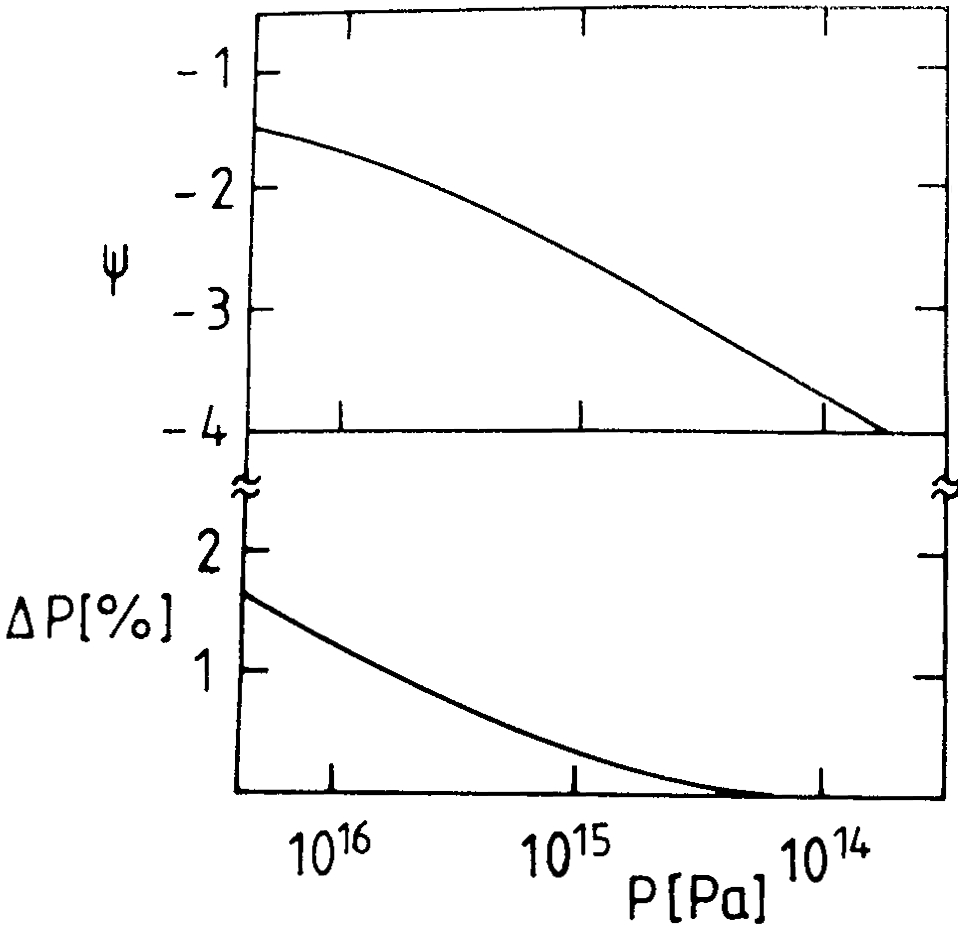
\includegraphics[width=0.9\textwidth,keepaspectratio]{degenpsiP}
\caption{Parametro di degenerazione $\Psi$ e correzioni alla pressione dovute alla degenerazione degli elettroni nell'interno solare.}
\end{subfigure}%
~
\begin{subfigure}[t]{0.5\textwidth}
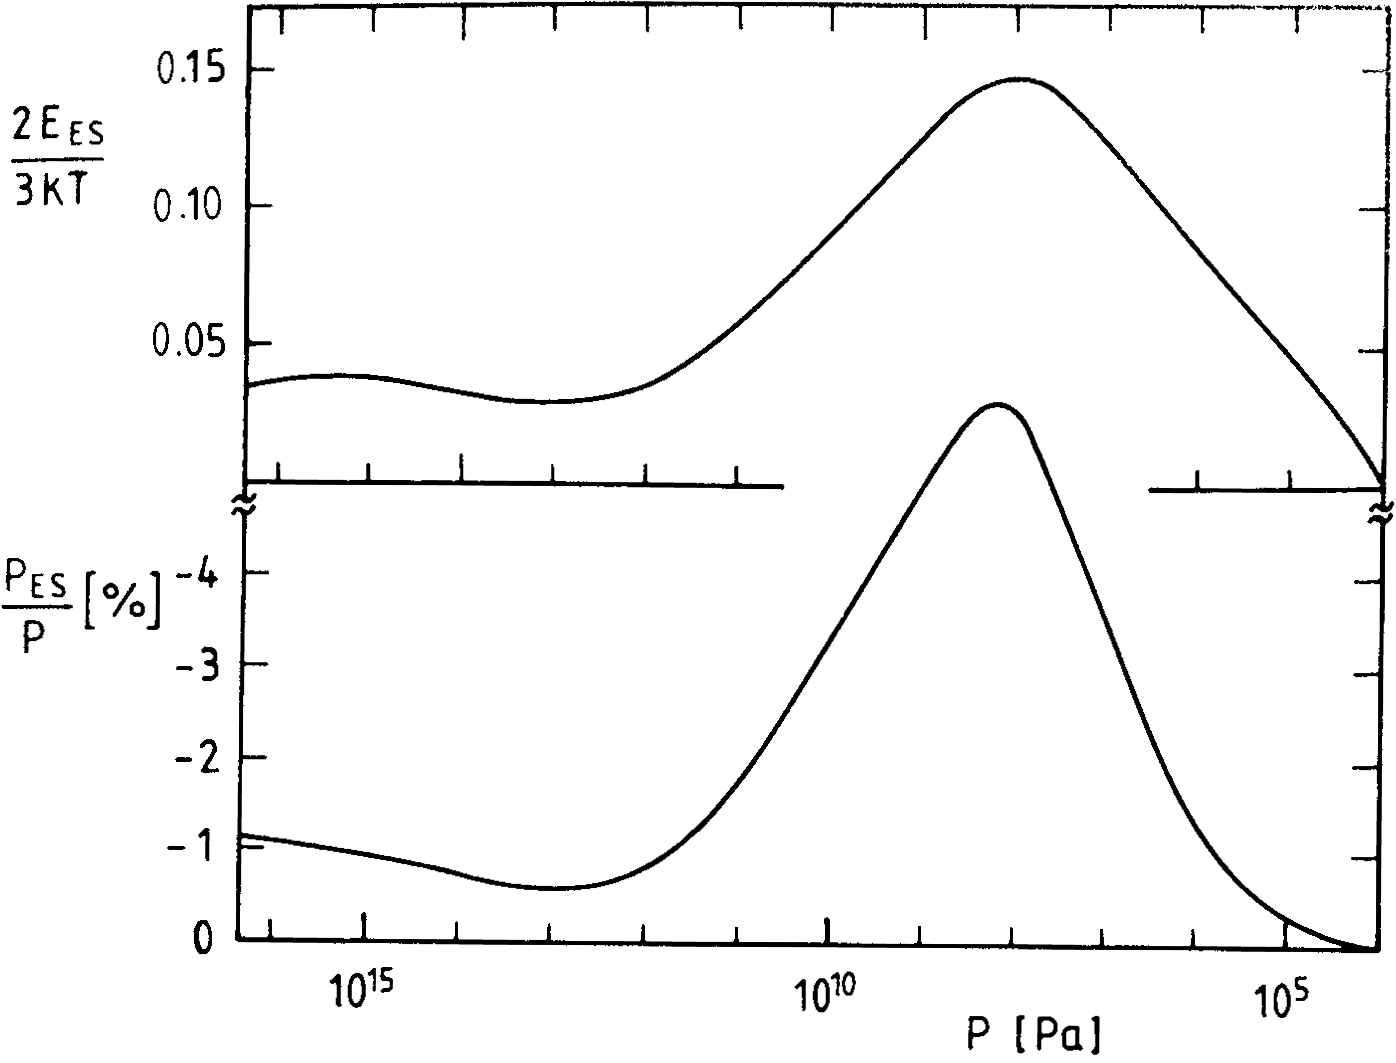
\includegraphics[width=0.9\textwidth,keepaspectratio]{RatioelectroEP}
\caption{Rapporto fra energia termica e coulombiana la prima e fra pressione e correzione coulombiana la seconda.}
\end{subfigure}
\end{figure*}

\item Interazioni coulombiane.

Introduco la correzione duvuta all'interazione Coulombiana secondo Debye-H\"uckel: il potenziale $V_i(r)$ dovuto allo ione $Z_i$ \'e schermato dagli elettroni quindi, per la formula di Boltzmann, la densit\'a degli ioni con carica Z \'e $n_Z=\overline{n}_Z\exp{-\frac{ZeV_i}{kT}}$, con $\overline{n}_Z$ densit\'a numerica dello ione $Z$ imperturbata. Assumendo l'energia coulombiana molto minore dell'energia termica espando $n_Z$ al prim'ordine quindi l'equazione di Poisson per $V_i$ \'e

\begin{align}
&\nabla^2V_i=-4\pi e\sum Zn_Z\approx\frac{1}{r_D^2}V_i\shortintertext{da cui ottengo il potenziale generato dalla nube di cariche attorno a Z}\nonumber\\
&\phi_Z=-\frac{eZ}{r_D}\shortintertext{dove}\nonumber\\
&\frac{1}{r_D^2}=\frac{4\pi e^2}{kT}\sum Z^2\overline{n}_Z=\frac{4\pi e^2}{kT}\zeta,\ \zeta=\sum_{i}(Z_i^2+Z_i)\frac{\rho X_i}{A_i}N_A\label{eq:debyeradius}
\end{align}

Le correzioni dovute alle interazioni coulombiane sono
\begin{align}
&u=\frac{3}{2}\frac{\gasconstant{}T}{\mu}+u_c,\ P=\frac{\rho}{\mu}kT+P_c\shortintertext{con}\nonumber\\[-2\normalbaselineskip]
&u_c=\frac{1}{2}\sum_ZeZ\overline{n}_Z\phi_Z=-e^3\sqrt{\frac{\pi\rho}{kT}}(N_A\zeta)\expy{\frac{3}{2}},\ P_c=\frac{1}{3}u_c
\end{align}

\end{itemize}


\section{Trasporto radiativo.}

Nell'interno stellare il cammino libero medio dei fotoni \'e molto corto $\frac{1}{\kappa\rho}\approx\SI{1}{\cm}\ll \rsun{}$, dove l'opacit\'a $\kappa$ che descrive l'assorbimento per unit\'a di massa, quindi considero la radiazione localmente in equilibrio con la materia: il flusso di energia verso la superficie \'e generato da una piccola anisotropia nell'intensit\'a descritta al prim'ordine tramite

\begin{equation}
I_{\nu}=B(\nu,T)-\frac{1}{\kappa_{\nu}'\rho}\nabla B(\nu,T)
\end{equation}

integrando sull'angolo solido, il flusso di energia risulta

\begin{align}
&\vec{F}_{\nu}=-\frac{4\pi}{3\kappa_{\nu}\rho}\nabla B(\nu,T)\shortintertext{ed esplicitando il gradiente termico e integrando sulle frequenze}\nonumber\\
&\vec{F}=-[\frac{4\pi}{3\rho}\intzi{}\frac{1}{\kappa_{\nu}}\PDy{T}{B(\nu,T)}\,d\nu]\nabla T\label{eq:radiativeflux}
\end{align}

Definisco l'opacit\'a media di Rosseland

\begin{equation}
\frac{1}{\kappa}=(\intzi{}\PDy{T}{B(\nu,T)})\expy{-1}\intzi{}\,d\nu\frac{1}{\kappa_{\nu}}\PDy{T}{B(\nu,T)}=(\frac{acT^3}{\pi})\expy{-1}\intzi{}\,d\nu\frac{1}{\kappa_{\nu}}\PDy{T}{B(\nu,T)}\label{eq:rosselandopacity}
\end{equation}

quindi riscrivo \eqref{eq:radiativeflux} utilizzando la pressione di radiazione $P_{rad}=\int\,d\nu\frac{4\pi}{3c}B_{\nu}=\frac{1}{3}aT^4$

\begin{align}
&\vec{F}=-\frac{4\pi}{3\kappa\rho}\nabla B=-\frac{4\pi}{3\kappa\rho}\nabla B=-\frac{c}{\kappa\rho}\nabla P_{rad}\shortintertext{che per una distribuzione sferica di materia diventa}\nonumber\\
&F_r=-\frac{c}{\kappa\rho}\TDof{r}(\frac{1}{3}aT^4)=-\frac{4acT^3}{3\kappa\rho}\TDy{r}{T}\label{eq:radfluxTgradrelation}
\end{align}

Definisco il gradiente radiativo a partire da \eqref{eq:radfluxTgradrelation}

\begin{equation}
\nrad{}=\Dcvar{\PDly{P}{T}}{rad}=\frac{3}{16\pi acG}\frac{\kappa l(r)P}{m(r)T^4}\label{eq:radiativegradient}
\end{equation}

con $l(r)=4\pi r^2F$ luminosit\'a totale in funzione di r.

\subsection{Opacit\'a.}

I fenomeni che contribuiscono all'opacit\'a nel Sole sono:

\begin{itemize}

\item \parbox[t]{\dimexpr\textwidth-\leftmargin}{%
\vspace{-2.5mm}
\begin{wrapfigure}{r}{0.5\textwidth}
\centering
\vspace{-\baselineskip}
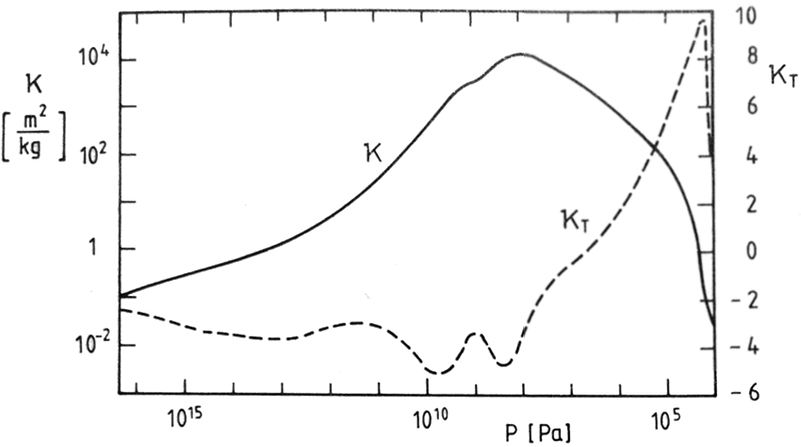
\includegraphics[keepaspectratio,width=0.9\linewidth]{opacitylld}
\caption{Profilo radiale di $\kappa$ e $\PDly{T}{\kappa}$. Da \cite{sti91sun}.}
\end{wrapfigure}


Scattering fotone-elettrone (sc). Classicamente \'e descritto come lo scattering di un'onda elettromagnetica piana da parte di un dipolo oscillante, scattering Thomson per $h\nu\ll m_ec^2$

\begin{align}
&\kappa_{\nu}\propto\frac{r_e^2}{\mu_em_u}, \kappa_{sc}=0.20(1+X)\si{\squared\cm\per\gram}\\
&r_e=\SI{2.82e-13}{\cm}
\end{align}

Per $T\geq\SI{e8}{\kelvin}$ il momento trasferito all'elettrone non \'e trascurabile, scattering Compton.

}

\item Brehmstrahlung inverso (ff). L'assorbimento di un fotone da parte di un elettrone libero \'e energeticamente possibile quando l'elettrone \'e vicino ad uno ione, l'opacit\'a in questo caso ha l'andamento

\begin{equation}
\kappa_{ff}\propto\rho T\expy{-\frac{7}{2}}
\end{equation}

si tiene conto degli effetti quantistici tramite un opportuno coefficiente, il fattore di Gaunt.

\item Reazioni di ionizzazione (bf).

\item Transizione elettronica a livelli eccitati (bb).

\item Scattering atomici e ione $H^-$. La presenza di metalli con potenziale di ionizzazione minore di H ed He rendono disponibile elettroni per la formazione di $H^-$, sistema debolmente legato per cui un fotone con $h\nu>\SI{0.75}{\ev}$ o $\lambda<\SI{1655}{\nano\meter}$ pu\'o essere assorbito.

\end{itemize}

La conduzione pu\'o essere trascurata in quanto nel Sole $l_{ph}\gg l_{e}$.


\begin{tikzpicture}[remember picture,overlay]

\node[anchor=south west] (opint) at ([shift={(0,2.5)}]current page.south west) {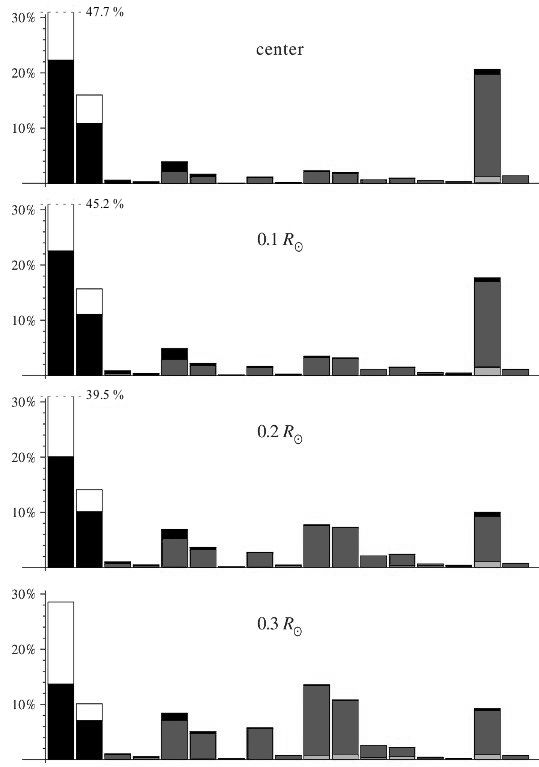
\includegraphics[width=0.55\textwidth,keepaspectratio]{opcontrib-int-g}};
\node[anchor=south east] (opout) at ([shift={(0,2.5-3/35)}]current page.south east) {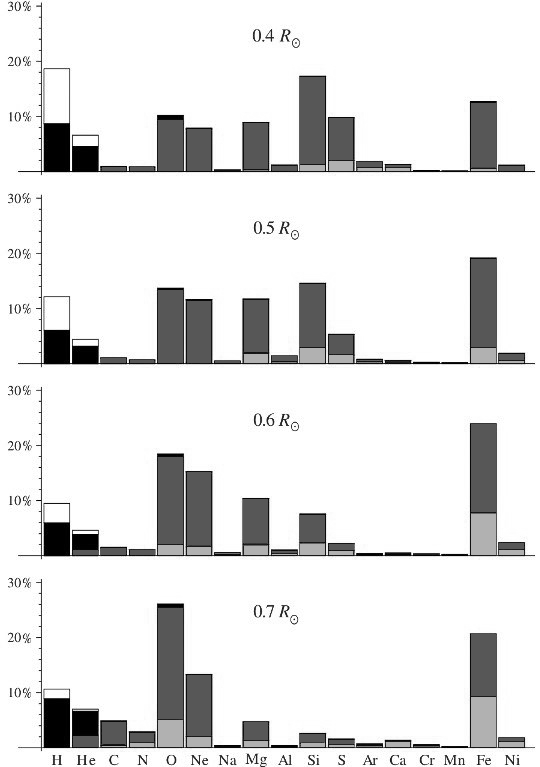
\includegraphics[width=0.55\textwidth,keepaspectratio]{opcontrib-out-g}};
\node[draw,anchor=south,label={[label distance=2mm]-90:Scattering \Pphoton\Pelectron},minimum size=5mm] (sc) at ([shift={(0,+7)}]current page.south) {};
\node[draw,label={[label distance=2mm]-90:ff},fill=black,minimum size=5mm,above=10mm of sc] (ff) {};
\node[draw,label={[label distance=2mm]-90:bb},fill=bb,minimum size=5mm,above=10mm of ff] (bb) {};
\node[draw,label={[label distance=2mm]-90:bf},fill=bf,minimum size=5mm,above=10mm of bb] (bf) {};


\node[name=hydrogen, right= 8mm of opint.south west] {\tiny H};
\node[name=helium, right=4.5mm of hydrogen.west] {\tiny He};
\node[name=carbonium, right=4.5mm of helium.west] {\tiny C};
\node[name=nitrum, right=4.5mm of carbonium.west] {\tiny N};
\node[name=oxygen, right=4.5mm of nitrum.west] {\tiny O};
\node[name=neon, right=4.5mm of oxygen.west] {\tiny Ne};
\node[name=sodium, right=4.5mm of neon.west] {\tiny Na};
\node[name=magnesium, right=4.5mm of sodium.west] {\tiny Mg};
\node[name=alluminium, right=4.5mm of magnesium.west] {\tiny Al};
\node[name=silicium, right=4.5mm of alluminium.west] {\tiny Si};
\node[name=sulfur, right=4.5mm of silicium.west] {\tiny S};
\node[name=argon, right=4.5mm of sulfur.west] {\tiny Ar};
\node[name=calcium, right=4.5mm of argon.west] {\tiny Ca};
\node[name=cromum, right=4.5mm of calcium.west] {\tiny Cr};
\node[name=manganese, right=4.5mm of cromum.west] {\tiny Mn};
\node[name=ferrum, right=4.5mm of manganese.west] {\tiny Fe};
\node[name=nikel, right=4.5mm of ferrum.west] {\tiny Ni};
\node[anchor=south west] at ([shift={(0,1.5)}]current page.south west) {\parbox{\textwidth}{\captionof{figure}{Importanza dei varii contributi all'opacit\'a nell'interno solare. Da \cite{bla11opacity}.}\label{fig:opacitycontrib} }};
 
\end{tikzpicture}

\clearpage

\section{Condizione di in-stabilit\'a dinamica: trasporto convettivo.}

La zona convettiva occupa il $29\%$ pi\'u esterno del raggio solare e contiene il $2\%$ della massa: questa regione \'e chimicamente omogenea. 

Una regione stellare \'e convettivamente stabile se una perturbazione radiale infinitesima non cresce ad ampiezza finita 
\begin{equation}
\rho\PtwoDy{t}{(\Delta r)}=-g\Delta\rho=-g[\Dcvar{\TDy{r}{\rho}}{e}-\Dcvar{\TDy{r}{\rho}}{amb}]\Delta r
\end{equation}

La forza di archimede ha verso opposta alla perturbazione se $\Delta\rho>0$.

Considero un'equazione di stato generica $\rho(P,T,\mu)$ e definita tramite:
\begin{align}
&\frac{d\rho}{\rho}=\alpha\frac{dP}{P}-\delta\frac{dT}{T}+\phi\frac{d\mu}{\mu}\label{eq:deltatherm}\\
&P=\frac{\rho\gasconstant{}T}{\mu}\quad\Rightarrow\quad\alpha=\delta=\phi=1
\end{align}

Suppongo il moto dell'elemento in equilibrio di pressione con l'ambiente quindi, definiti i gradienti termici per il blob e l'ambiente e il gradiente di composizione chimica 

\begin{equation}
\nabla=\Dcvar{\TDly{P}{T}}{amb},\ \nabla_e=\Dcvar{\TDly{P}{T}}{blob},\ \nmu{}=\Dcvar{\TDly{P}{\mu}}{amb}\label{eq:nablavitense}
\end{equation}
riscrivo l'equazione del moto utilizzando l'equazione di stato, essendo $\nmu{}_{blob}\approx0$,
\begin{equation}
\PtwoDy{t}{(\Delta r)}=-g\frac{\delta}{H_P}[\nabla_e-\nabla-\frac{\phi}{\delta}\nmu{}]\Delta r\label{eq:galleggiamento}
\end{equation}

Suppongo adesso un moto del blob adiabatico $\nabla_e=\nabla_{ad}=\frac{P\delta}{T\rho c_P}$ e introduco la frequenza di \bv{}:
\begin{align}
&N^2=g(\frac{1}{\Gamma_1P}\TDy{r}{P}-\frac{1}{\rho}\TDy{r}{\rho})\label{eq:bvfs}\\
&N^2=g(\frac{1}{\densityscale{}}-\frac{g}{c_s^2})\label{eq:bvfsdensita}\shortintertext{ho definito le lunghezze caratteristiche per variazione di densit\'a e pressione:}\nonumber\\
&\densityscale{}=-\frac{dr}{d\ln{\rho}},\ H_P=-\frac{dr}{dP}
\end{align}

$N^2$ rappresenta la massima frequenza sotto cui pu\'o oscillare una particella di fluido sottoposta a onde di gravit\'a mantenendo l'equilibrio di pressione con l'ambiente.

Riscrivo l'equazione \eqref{eq:galleggiamento}
\begin{equation}
\PtwoDy{t}{(\Delta r)}=-N^2\Delta r
\end{equation}
che descrive un comportamento oscillatorio per $N^2>0$, cio\'e uno strato di gas del Sole \'e stabile per convezione se

\begin{equation}
\nrad{}<\nad+\frac{\phi}{\delta}\nmu{}\label{eq:ledoux}
\end{equation}

dove ho usato $\nabla_{amb}=\nrad{}$ definito in \eqref{eq:radiativegradient}, cio\'e il gradiente che si ha nel caso la luminosit\'a si trasportata dai fotoni.

Le basse temperature causano un aumento dell'opacit\'a e il gradiente termico necessario per trasportare la luminosit\'a solare \'e superiore al gradiente adiabatico, il cui valore \'e diminuito dal calore latente dell'idrogeno solo parzialmente ionizzato.

Una maggiore efficienza del trasporto convettivo di energia si riflette in una minore differenza tra il gradiente di temperature adiabatico ed effettivo.

\begin{figure}[!h]
\begin{subfigure}[l]{0.55\textwidth}
    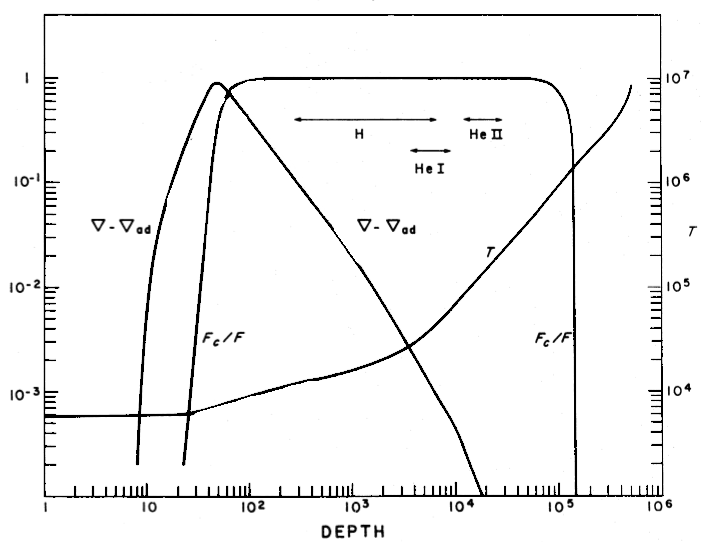
\includegraphics[ width=0.99\textwidth,keepaspectratio]{proportionflux}
    \caption{Profilo radiale del flusso convettivo rispetto al flusso totale, della super-adiabaticit\'a del gradiente termico e regioni di ionizzazione parziale di $\cel{He}{4}{}{}$. Da \cite{gou76convection}}
    \label{fluxproportion}
\end{subfigure}
~
\begin{subfigure}[r]{0.4\textwidth}
\centering
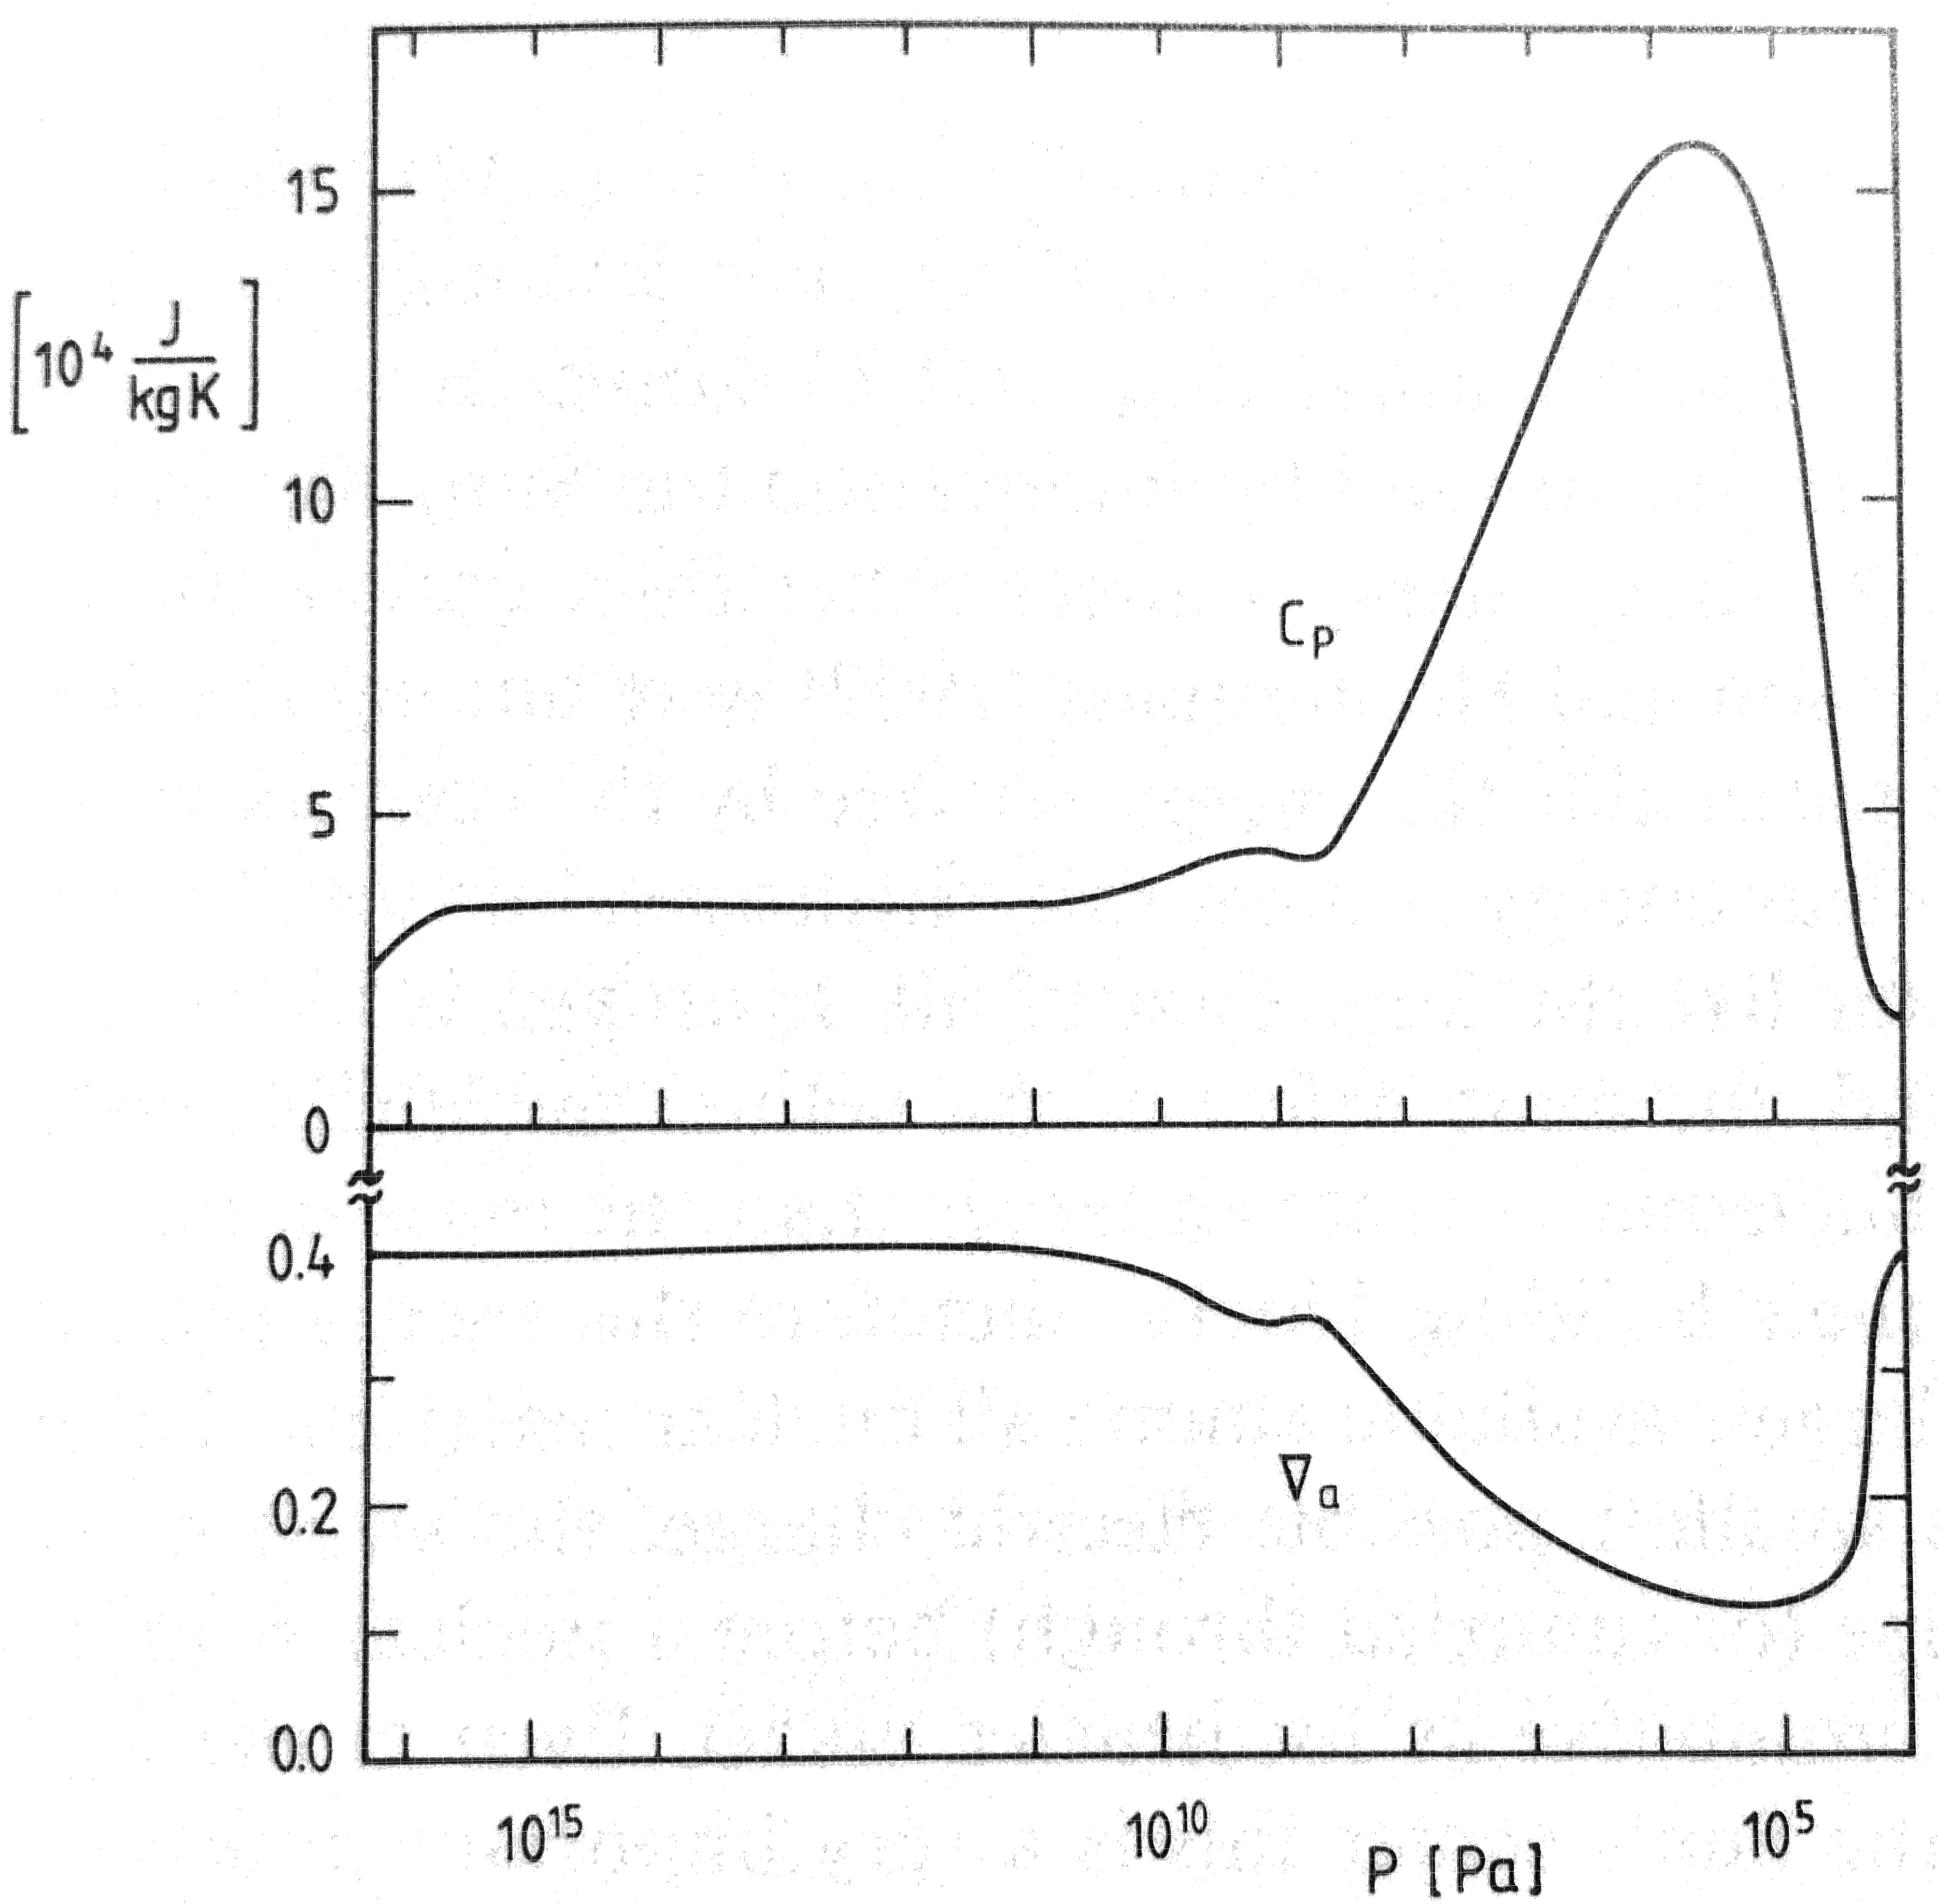
\includegraphics[keepaspectratio,width=0.9\textwidth]{specificheatnablaa}
\subcaption{Profilo radiale di $c_P$ e $\nabla_a$. Da \cite{sti91sun}.}
\end{subfigure}
    
\end{figure}


\subsection{Teoria della mixing-length.}

Il flusso di energia complessivo \'e determinato da
\begin{equation}
F_{con}+F_{rad}=\frac{4acG}{3}\frac{T^4m}{\kappa Pr^2}\nrad{}\label{eq:totalflux}
\end{equation}

Per determinare il gradiente di temperatura effettivo $\nabla$ uso la teoria della mixing-length (\cite{prandtl25tur} e \cite{vitense53kon}):
si considera l'eccesso di calore trasportato dai blob di gas nel moto convettivo $c_P\Delta T$ rispetto all'ambiente, il cui cammino libero medio \'e la mixing-length $l_m=\alpha H_P$, che da luogo al flusso di energia

\begin{equation}
F_{con}=\exv{\rho vc_P\Delta T}\label{eq:convectiveflux}
\end{equation}

dove $\exv{}$ indica una media opportuna sul guscio sferico di raggio r. Determino il valor medio della differenza di temperatura prendendo come valore caratteristico dello spostamento del blob di gas $\Delta r\approx\frac{l_m}{2}$:

\begin{equation}
\frac{\Delta T}{T}\approx\frac{1}{T}\PDy{r}{(\Delta T)}\frac{l_m}{2}=(\nabla-\nabla_e)\frac{l_m}{2}\frac{1}{H_P}
\end{equation}

Assumo il lavoro medio fatto dalla forza di galleggiamento per unit\'a di massa $-g\frac{\Delta\rho}{\rho}$ uguale al valore medio della forza, cio\'e la met\'a di quello al guscio sferico dato, moltiplicato lo spostamento medio $\frac{l_m}{2}$ quindi, assumendo in oltre che in media met\'a del lavoro fatto dalla forza di galleggiamento sia trasformato in energia cinetica del blob si ottiene

\begin{equation}
v^2=g\delta(\nabla-\nabla_e)\frac{l_m^2}{8H_P}\label{eq:blobvelocity}
\end{equation}

Infine determino gli scambi radiative del blob: il modulo del flusso radiativo \'e proporzionale al gradiente termico in direzione normale alla superficie del blob

\begin{equation}
f=\frac{4acT^3}{3\kappa\rho}|\PDy{n}{T}|
\end{equation}

quindi l'energia scambiata dall'intera superficie S del blob \'e $\lambda=Sf$ che determina, per la prima legge della termodinamica, una variazione di temperatura per unit\'a di tempo, indicato con $V$ il volume, $\PDy{t}{T_e}=-\frac{\lambda}{\rho Vc_P}$.

La variazione della temperatura del blob per unit\'a distanza percorsa \'e quindi
\begin{equation}
\Dcvar{\TDy{r}{T}}{e}=\Dcvar{\TDy{r}{T}}{ad}-\frac{\lambda}{\rho Vc_Pv}\label{eq:Tchangelength}
\end{equation}
esplicitando $\lambda$, approssimando il gradiente normale alla superficie con $\exv{\Delta T}$ ed usando le definizioni \eqref{eq:nablavitense} si ottiene
\begin{equation}
\frac{\nabla_e-\nad{}}{\nabla-\nabla_e}=\frac{6acT^3}{\kappa\rho^2c_Pl_mv}
\end{equation}

Le 5 equazioni \eqref{eq:totalflux},\eqref{eq:radiativegradient}, \eqref{eq:convectiveflux}, \eqref{eq:blobvelocity}, \eqref{eq:nablavitense} determinano completamente le variabili $F_{rad}, F_{con}, v, \nabla_e, \nabla$ in funzione di $P,T,l(r),m(r),c_P,\nad{},\nrad{},g$ .


\section{Reazioni di fusione.}

L'energia liberata dalle reazioni nucleari per grammo per secondo $\epsilon(\rho,T,X_i)$ \'e determinata dalla probabilit\'a che la reazione $X(a,b)Y$ abbia luogo. Sia $E$ l'energia cinetica nel centro di massa dei nuclei, per la sezione d'urto $\sigma(E)$ di fusione si ha

\begin{align}
&\sigma(E)\propto\pi\lambdabar^2P_0(E)\xi(E)&\intertext{La lunghezza d'onda di de Broglie relativa delle particelle descrive l'indeterminazione sulla posizione nell'urto di due particelle con momento relativo p}\nonumber\\
&\lambdabar=\frac{\hbar}{p}=\frac{\hbar}{\sqrt{2mE}}&\intertext{$\xi(E)$ tiene conto di eventuali livelli risonanti: $\xi(E)\to1$ lontano dall'energia del livello risonante. $P_0(E)$ descrive la probabilit\'a di attraversamento della barriera coulombiana. Introducendo il fattore astrofisico, dipendente dalle caratteristiche dei nuclei e debolmente dall'energia lontano da risonanze, scrivo la sezione d'urto per i nuclei di carica $Z_1$, $Z_2$ e m massa ridotta}\nonumber\\
&\sigma(E)=\frac{S(E)}{E}\exp{-2\pi\eta},\ \eta=\sqrt{\frac{m}{2}}\frac{Z_1Z_2e^2}{\hbar E\expy{\frac{1}{2}}}
\end{align}

La funzione $\epsilon(\rho,T,X_i)$ \'e determinata dalla somma di tutti i contributi

\begin{equation}
\epsilon_{ij}=\frac{1}{1+\delta_{ij}}\frac{Q_{ij}}{m_jm_k}X_jX_k\exv{\sigma v}\label{eq:energyrate}
\end{equation}

dove $Q_{ij}$ \'e l'energia liberata per reazione tra nucleo di specie i e j; $\exv{}$ indica la media sulla distribuzione di Maxwell-Boltzmann

\begin{equation}
f(E)dE\propto\frac{E\expy{\frac{1}{2}}}{(kT)\expy{\frac{3}{2}}}\exp{-\frac{E}{kT}}\,dE
\end{equation}

\begin{figure*}[!h]
    \centering
  \begin{subfigure}[t]{0.6\textwidth}
        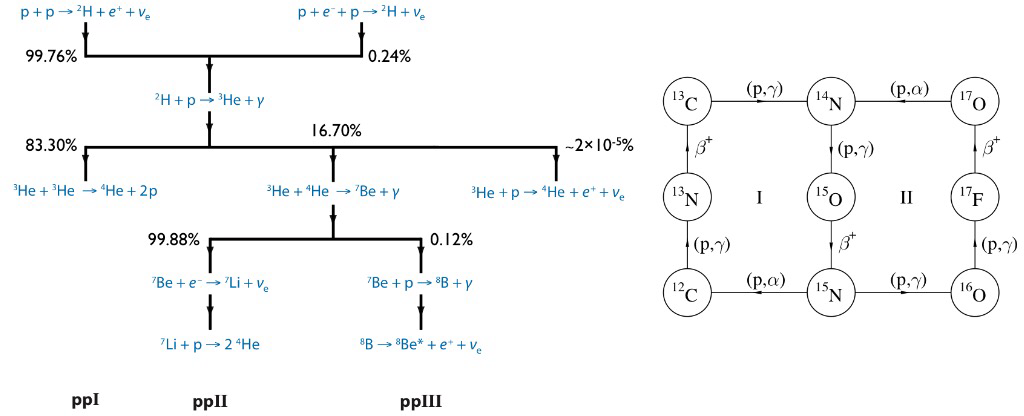
\includegraphics[width=0.9\textwidth,keepaspectratio]{ReactionsH}
        \caption{Reazioni di fusione H-He: catena PP e ciclo CNO.}
    \end{subfigure}%
    ~
    \begin{subfigure}[t]{0.4\textwidth}
        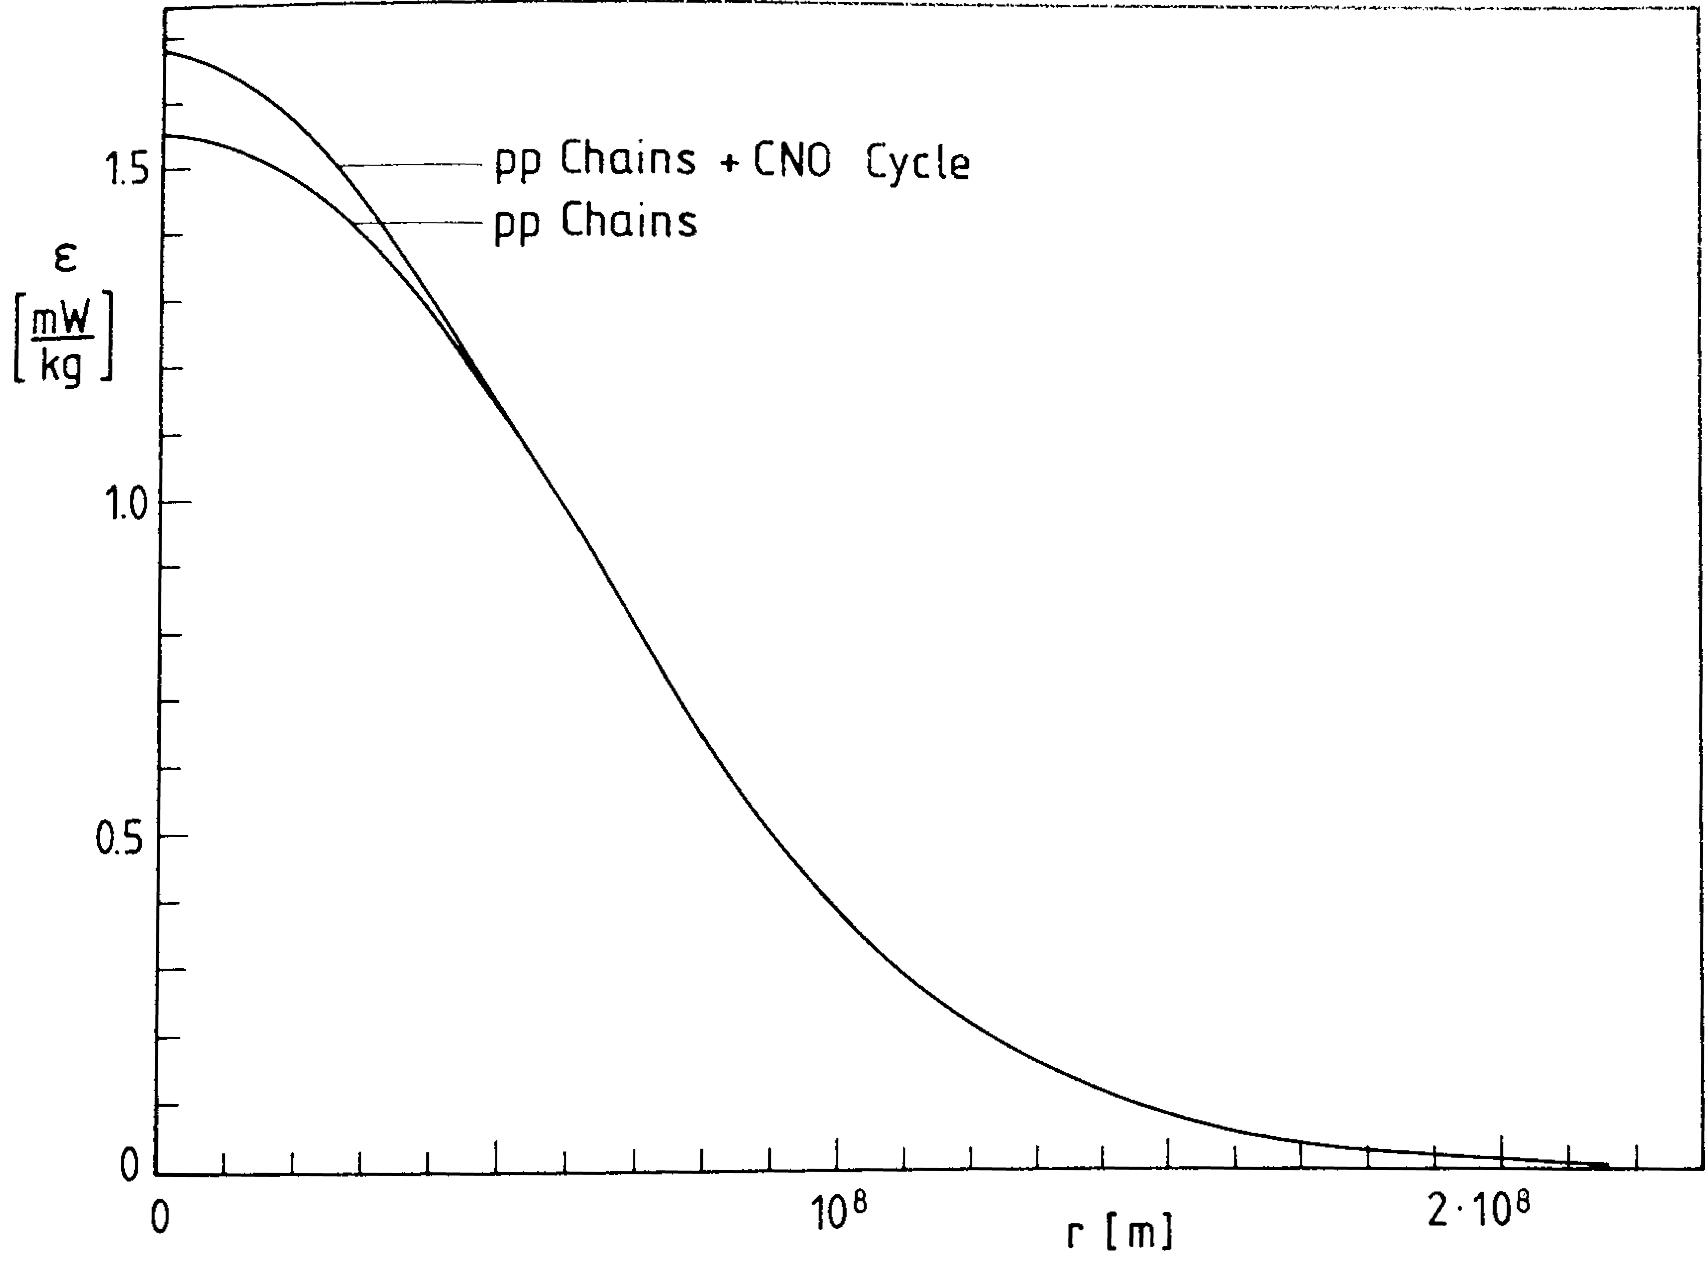
\includegraphics[width=0.9\textwidth,keepaspectratio]{watt-PPvsCNO}
        \caption{Andamento della luminosit\'a nel Sole.}
    \end{subfigure}
\end{figure*}

Per determinare $\exv{\sigma v}$ uso il fatto che l'integrando $S(E)\exp{-\frac{E}{kT}-\frac{b}{\sqrt{E}}}$ ha forma approssimativamente gaussiana il cui massimo $E_0$, energia pi\'u probabile di reazione, e FWHM sono, posto $A=Z_j^2Z_k^2A=Z_j^2Z_k^2\frac{A_iA_j}{A_i+A_j}$:
\begin{align}
&E_0=\SI{5.665}{\kilo\ev} A\expy{\frac{1}{3}}T_7\expy{\frac{2}{3}},\ \Delta E=4.249W\expy{\frac{1}{6}}T_7\expy{\frac{5}{6}}&\intertext{quindi il rate locale per reazioni non risonanti si scrive}\\
&\exv{\sigma v}=\num{1.3005e-15}[\frac{Z_1Z_2}{AT_6^2}]\expy{\frac{1}{3}}fS_{eff}\exp{-\tau}\si{\cubic\cm\per\second},\ \tau=\frac{3E_0}{kT}\approx\num{42.487}(Z_1^2Z_2^2AT_6\expy{-1})\expy{\frac{1}{3}}&\intertext{$S_{eff}$ \'e il risultato dell'espansione dell'integrando per $\invers{\tau}\ll1$ ed estrapolato a $E_0$ a partire dal valore a $E(0)$ determinato dalla fisica nucleare.}
\end{align}

Lo schermaggio degli elettroni diminuisce la repulsione coulombiana e analogamente a quanto visto in precedenza si ha:
\begin{equation}
E_C'-E=\frac{Z_1Z_2e^2}{r}\exp{-\frac{r}{r_D}}-E\approx\frac{Z_1Z_2e^2}{r}-\frac{Z_1Z_2e^2}{r_D}-E=E_C-E-E_D
\end{equation}

Per $\frac{E_D}{kT}\ll1$ ne tengo conto aggiungendo il parametro correttivo $f$
\begin{equation}
\exv{v\sigma}\to f\exv{v\sigma},\ f=\exp{\frac{E_D}{KT}}
\end{equation}

% T_6=10T_7=10^3T_9

\begin{figure*}[!h]
    \centering
  \begin{subfigure}[t]{0.5\textwidth}
        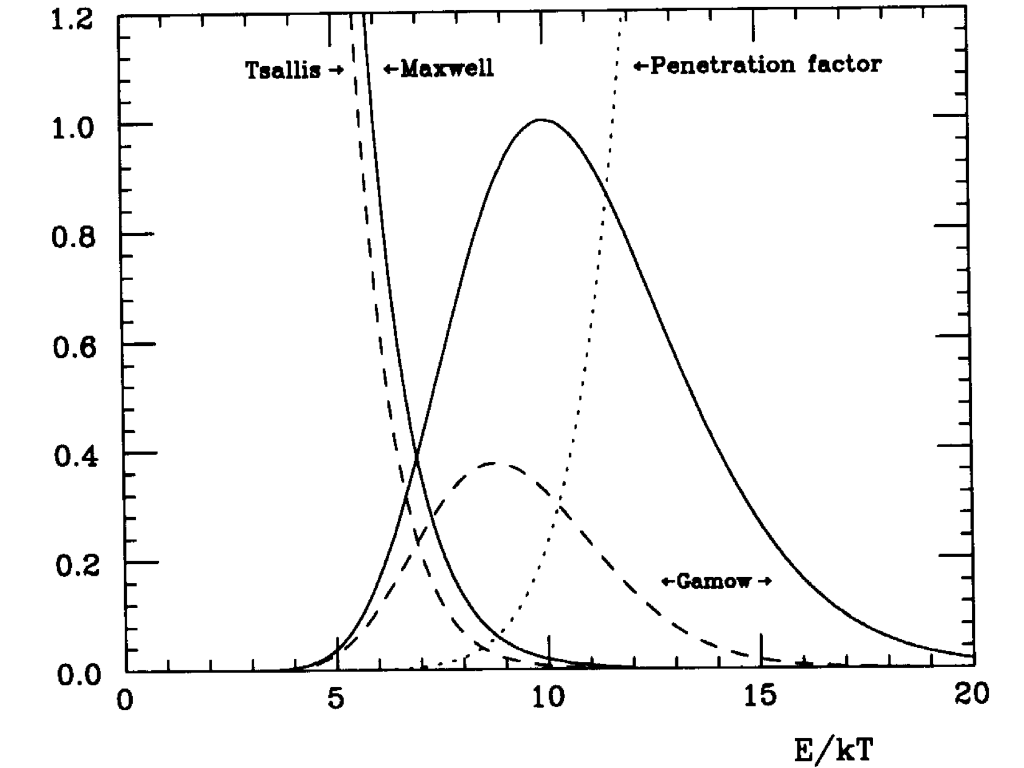
\includegraphics[width=0.9\textwidth,keepaspectratio]{gamow}
        \caption{Picco di Gamow per distribuzione velocit\'a nuclei MB a T.}
    \end{subfigure}%
    ~
    \begin{subfigure}[t]{0.5\textwidth}
        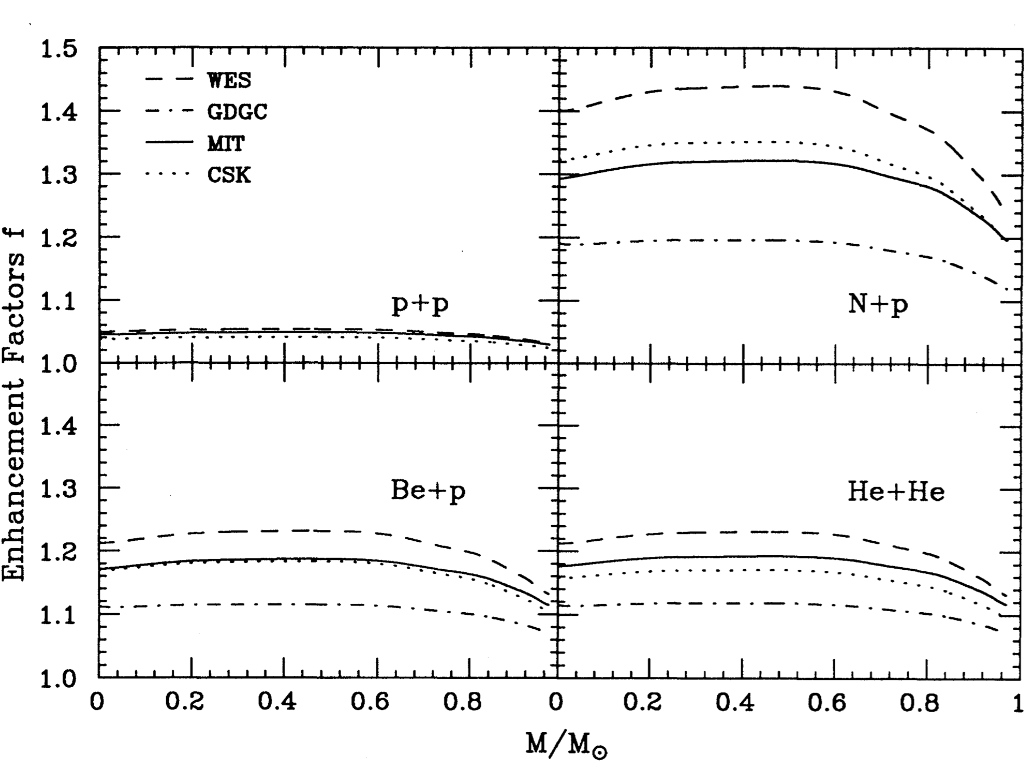
\includegraphics[width=0.9\textwidth,keepaspectratio]{Rscreening}
        \caption{Andamento della correzione di schermaggio degli elettroni.}
    \end{subfigure}
\end{figure*}

\begin{comment}
\begingroup
\color{grey}
La composizione chimica \'e modificata dalle reazioni di fusione che per gli elementi principali, assumendo condizione di equilibrio secolare, riassumo
%%% \tag{\theequation a,b}
\begin{subequations}\label{subeqn:fusionchange}
\begin{align}
&\dot{X}=\frac{m_p}{N_A}(-3r_{pp}+2r_{33}-r_{34}-4r_{p14})\\ 
&\dot{Y}_3=\frac{m_{He3}}{N_A}(r_{pp}-2r_{33}-r_{34})\\
&\dot{Y}=\frac{m_{He4}}{N_A}(r_{33}+r_{34}+r_{p14})
\end{align}
\end{subequations}

con $r_{ik}$ rate di reazione per unit\'a di massa:

\begin{align}
&r_{ik}=\frac{\rho N_A^2X_iX_k}{(1+\delta_{ik})A_iA_k}\lambda_{ik}\shortintertext{dove, introducendo il fattore astrofisico $S(E)$, la massa ridotta dei due reagenti $m_{ik}$}\nonumber\\
&\lambda_{ik}=\sqrt{\frac{8}{m_{ik}\pi}}\frac{S_{ik}|_{E=0}}{(kT)\expy{\frac{3}{2}}}\intzi{}\exp{(-\frac{E}{kT}-\frac{b}{\sqrt{E}})}\,dE,\ b=31.28Z_1Z_2\sqrt{\frac{m_{ik}}{m_u}}\,(KeV)\expy{-1}\label{eq:astrofactor}
\end{align}

\endgroup

\end{comment}

\section{Composizione chimica e processi di diffusione.}

La composizione chimica del Sole \'e determinata analizzando le righe di assorbimento prodotte dalle transizioni atomiche negli strati esterni del Sole; poich\'e l'assorbimento continuo \'e dovuto principalmente all'idrogeno l'abbondanza degli elementi pesanti si esprime relativamente all'abbondanza di idrogeno.

%La composizione chimica \'e modificata dalle reazioni di fusione che per gli elementi principali, assumendo condizione di equilibrio secolare, riassumo
%%% \tag{\theequation a,b}
%\begin{subequations}\label{subeqn:fusionchange}
%\begin{align}
%&\dot{X}=\frac{m_p}{N_A}(-3r_{pp}+2r_{33}-r_{34}-4r_{p14})\\ 
%&\dot{Y}_3=\frac{m_{He3}}{N_A}(r_{pp}-2r_{33}-r_{34})\\
%&\dot{Y}=\frac{m_{He4}}{N_A}(r_{33}+r_{34}+r_{p14})
%\end{align}
%\end{subequations}
%con $r_{ik}$ rate di reazione per unit\'a di massa.

La composizione iniziale del Sole, supposta omogenea, \'e determinata a partire dalla composizione attuale delle regioni esterne, tenendo conto della diffusione, e attraverso la calibrazione del modello solare per le abbondanze di $\cel{H}{1}{}{}$ e $\cel{He}{4}{}{}$.


\begin{table}[!h]

\pgfplotstabletypeset[
every head row/.style={
 before row={\toprule &\multicolumn{4}{c|}{Attuale}&\multicolumn{4}{c|}{Primordiale}\\\midrule},
 every last row/.style={after row=\bottomrule},
 after row={\midrule}
},
every last row/.style={after row=\bottomrule},
every first column/.style={column type/.add={|}{}},
every last column/.style={column type/.add={}{|}},
columns/x/.style = {column type/.add={|}{}},
columns/xi/.style = {column type/.add={|}{}},
display columns/0/.style={column name={}},
display columns/1/.style={column name={$X$}},
display columns/2/.style={column name={$Y$}},
display columns/3/.style={column name={$Z$}},
display columns/4/.style={column name={$\frac{Z}{X}$}},
display columns/5/.style={column name={$X$}},
display columns/6/.style={column name={$Y$}},
display columns/7/.style={column name={$Z$}},
display columns/8/.style={column name={$\frac{Z}{X}$}},
create on use/authors/.style={create col/set list={Anders \& Grevesse (1989),Grevesse \& Noels (1993),Grevesse \& Sauval (1998),Lodders (2003),Asplund Grevesse \& Sauval (2005),Lodders Palme \& Gail (2009),\cite{asplund2009chemical}}},
columns/authors/.style={string type},
columns={authors,x, y, z, zx,xi,yi,zi, zxi},
/pgf/number format/precision=4
     ]{asplund.txt} %%%attuale

\captionof{table}{Metallicit\'a osservata e iniziale. Da \cite{asplund2009chemical}.}
\end{table}
 
%\begin{minipage}{0.5\textwidth}
%\begin{table}
%     \pgfplotstabletypeset[
%every head row/.style={
%before row={\toprule &\multicolumn{4}{c}{Iniziale}\\},
%},
%every last row/.style={after row=\bottomrule},
%display columns/0/.style={column name={$X$}},
%display columns/1/.style={column name={$Y$}},
%display columns/2/.style={column name={$Z$}},
%display columns/3/.style={column name={$\frac{Z}{X}$}},
%columns={x, y, z, zx},
%/pgf/number format/precision=4
%    ]{asplundprimordial.txt}.  %%% Iniziale

%Oltre alle reazioni di fusioni anche i processi di diffusione modificano l'abbondanza degli elementi, il peso molecolare medio e l'opacit\'a.

L'equazione di Boltzmann del trasporto descrive l'evoluzione della probabilit\'a $f(\vec{r},\vec{v},t)$ che una particella di una determinata specie sia in una regione dello spazio delle fasi.

\begin{align}
&\PDy{t}{f_i}+\vec{v}_i\cdot\PDy{\vec{r}}{f_i}+\vec{F}_i\cdot\PDy{\vec{v}}{f_i}=-\nabla_{\vec{p}}(\vec{s}),\ 
s_{\alpha}=\sum_{'}\int [f(\vec{p})\PDy{p'_{\beta}}{f'(\vec{p}'}-f'(\vec{p}')\PDy{p_{\beta}}{f(\vec{p})}]B_{\alpha\beta}\,d^3p'&\intertext{$\vec{s}$ \'e il flusso nello spazio dei momenti dovuto alle collisioni, la somma \'e sulle specie diverse da i e}\nonumber\\
&B_{\alpha\beta}=\frac{1}{2}\int q_{\alpha}q_{\beta}|\vec{v}-\vec{v}'|\,d\sigma,\ 
d\sigma=\frac{4\pi(Z_iZ_j)^2}{\mu^2(\vec{v}-\vec{v}')^4}\frac{d\chi}{\chi^3}&\intertext{con $d\sigma$ sezione d'urto differenziale per potenziale coulombiano puro per piccoli angoli, $\chi$ deviazione nel sistema CM e $\mu$ massa ridotta e}\nonumber\\
&\sigma_{st}=\frac{4\pi(Z_sZ_t)^2}{\mu^2(\vec{v}-\vec{v}')^4}L,\ L=\ln{\frac{1}{\chi_{min}}}=\ln{\frac{\lambda\mu v_{rel}^2}{|Z_sZ_t|^2}}
\end{align}

Il plasma solare \'e costituito principalmenteda $\cel{H}{1}{}{}$, $\cel{He}{4}{}{}$, \Pelectron e in minore abbondanza nuclei pesanti.

 La distribuzione di velocit\'a della specie i \'e approssimativamente la distribuzione di equilibrio traslata di $w^i$.

Per la velocit\'a di diffusione relative dei due elementi pi\'u abbondanti, definita la concentrazione relativa $c_i=\frac{n_i}{n}$ e il coefficiente di diffusione $D_{HHe}=-\frac{1}{3}lv_{th}$ con $l\approx(n\sigma)\expy{-1}$ cammino libero medio

\begin{align}
&w_H-w_{He}=\frac{1}{n_H}\int\,d^3v_Hf_H\vec{v}_H-\frac{1}{n_{He}}\int\,d^3v_{He}f_{He}\vec{v}_{He}\\
&=-D_{HHe}\left[\frac{1}{c_Hc_{He}}\PDy{r}{c_H}+\frac{m_{He}-m_H}{c_Hm_H+c_{He}m_{He}}\frac{1}{P}\PDy{r}{P}+\frac{K_T}{n_Hn_{He}}\frac{1}{T}\PDy{r}{T}\right]
\end{align}

La forza per unit\'a di volume agente sulle particelle di specie i \'e

\begin{align}
&\vec{F}_i=-\nabla P_i+n_i(q_i\vec{E}+m_i\vec{g})&\intertext{e in condizioni di equilibrio il momento trasferito tramite urti con le altre specie \'e}\nonumber\\
&\vec{F}_i=\sum_{i\neq j}\vec{F}_{ij},\ \vec{F}_{ij}=m_{ij}n_in_j\sigma_{ij}\vec{v}_{ij}&\intertext{dove la funzione $w_{ij}$ \'e la sezione d'urto di Rutherford per la velocit\'a media relativa delle particelle $i,j$}\nonumber\\
&\sigma_{ij}=\num{2.68e-12}Z_i^2Z_j^2(\frac{m_{ij}}{m_H})\expy{-\frac{1}{2}}(\frac{T}{\SI{e7}{\kelvin}})\expy{-\frac{3}{2}}\ln{\lambda_{ij}}\si{\cubic\cm\per\second}
\end{align}

Il momento trasferito dagli ioni agli elettroni \'e piccolo quindi si ha

\begin{align}
&F_H\approx F_{HHe}=-\PDy{r}{P_H}+n_H(eE+m_Hg)\\
&F_{He}\approx -F_{HHe}=-\PDy{r}{P_{He}}+n_{He}(2eE+4m_Hg)\\
&E=-\frac{1}{en_e}\PDy{r}{P_e}&\intertext{Per le velocit\'a di diffusione si ha}\nonumber\\
&w_{HHe}=-\frac{m_{He}T}{m_{HHe}Y\rho \sigma_{HHe}}[\PDy{r}{\ln{(P_eP_H)}}-m_Hg],\ 
n_Hw_H=\frac{(m_{He}n_Hn_{He})}{\rho}w_{HHe}\\
&w_A(1+2\frac{Y}{X})\approx-w_H
%&n_Av_A(m_{AH}n_Hw_{AH})(1+2\frac{Y}{X})\approx-n_Av_H(m_{AH}n_Hw_{AH})
\end{align}

La gravit\'a tende a concentrare gli elementi pi\'u pesanti verso il centro, le interazioni elettromagnetiche mantengono gli elettroni ancorati ai nuclei mentre $\nabla P_i$ contiene un contributo dovuto a $\nabla n_i$ che tende a diminuire il gradiente di concentrazione.
 
La diffusione termica concentra le particelle pi\'u cariche e pi\'u pesanti nelle zone pi\'u calde: infatti la presenza di un gradiente termico determina un flusso di calore, dovuto al maggior numero di particelle energetiche provenienti dalle regioni pi\'u calde, principalmente nuclei di idrogeno, e la  diversa probabilit\'a di trasferimento di momento negli urti nella direzione del gradiente, la sezione d'urto coulombiana dipende dalla velocit\'a relativa $\propto v\expy{-4}$ probabilit\'a di collisione $\propto v\expy{-3}$), produce una forza nel verso opposto al gradiente termico sugli ioni di idrogeno ed una opposta sugli ioni di elio.

\begin{align}
&\vec{q}_i=\int\frac{1}{2}m_iv_i^2\vec{v}_in_if_i\,d^3v_i\approx-\frac{5}{2}\frac{P_i\tau_ik}{m_i}\nabla T\\
&\overline{\nu}=\frac{1}{3}\int f^{(0)}\frac{m_{HHe}g^2}{kT}\nu(g)\,d^3g\\
&\vec{w}_{HHe}^{th}\approx\frac{2}{5kN_Hn_{He}}(\frac{n_{He}m_{He}\vec{q}_H-n_Hm_H\vec{q}_{He}}{m_H+m_{He}})\PDy{T}{\ln{\overline{\nu}}}
\end{align}

%Si tiene conto del flusso di massa, momento ed energia nelle equazioni di conservazione attraverso le equazioni sviluppate da Burgers (1969).

\begin{minipage}{\linewidth}
\begin{tikzpicture}
\node[inner sep=0pt] (image) at (0,0)
  {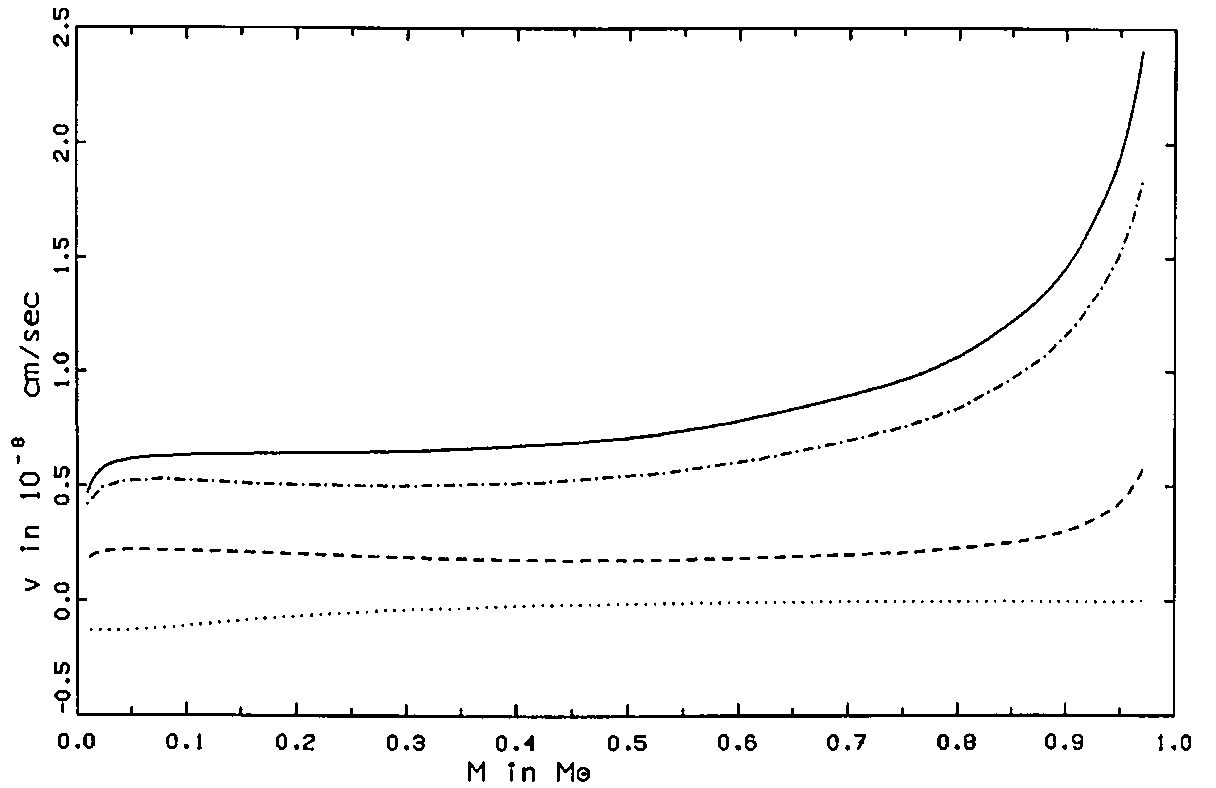
\includegraphics[keepaspectratio=true,width=0.5\textwidth]{Hdiffusion}};
  \draw [thick,dotted] (-3.4,1.5) -- (-3,1.5) node[right] {$\propto\nabla c$};
 \draw [thick,dashed] (-3.4,1.9) -- (-3,1.9) node[right] {$\propto\nabla T$};
    \draw [thick,dash dot] (-3.4,2.3) -- (-3,2.3) node[right] {$\propto\nabla P$};
    \node (caption) at (8.5,-2.5) { \begin{minipage}[c]{0.48\textwidth}
\captionof{figure}{Contributi alla velocit\'a di diffusione di H-He in modello di $1\msun{}$ a \SI{4.65e9}{\year}. Da \cite{wam88hydrogen}.}%   
    \end{minipage}};
\node[] (massconsdiff) at (8.5,1) {\begin{minipage}[c]{0.48\textwidth}

Sebbene il tempo caratteristico per percorre un raggio solare sia lungo $\tau_{diff}\approx\SI{6e13}{\year}$ i processi di diffusione producono effetti misurabili sulle frequenze dei modi di oscillazione: la loro inclusione nei \mss{} produce un miglior accordo con le osservazioni.

\end{minipage}
};
\end{tikzpicture}
\end{minipage}


% $D_{12}$ vs $K_T=\alpha n_0n_1$ thermal diffusion ration. Thermal diffusion coefficient: $D_T=D_{12}K_T$


\section{Modello di Sole attuale.}

Determino la struttura solare integrando numericamente le equazioni fondamentali della struttura stellare
\begin{subequations}\label{subeqn:stellarstructure}
\begin{align}
&\TDy{r}{m}=4\pi r^2\rho\\
&\TDy{r}{P}=-\frac{Gm(r)\rho(r)}{r^2}\\
&\TDy{r}{T}=\nabla\frac{T}{p}\TDy{r}{p}\\
&\TDy{r}{L}=4\pi r^2[\rho(\epsilon-\epsilon_{\nu})-\rho\TDof{t}u+\frac{P}{\rho}\TDy{t}{\rho}]
\end{align}

\begin{equation}
\PDy{t}{n_s}+\frac{1}{r^2}\PDof{r}(r^2n_sw_s)=\Dcvar{\PDy{t}{n_s}}{Nucl}\label{eq:difffusionchange}
\end{equation}
\end{subequations}
con $w_s$ velocit\'a di diffusione specie s. Ottengo il profilo radiale delle grandezze $\{P,m,T,L,X_i\}$, note  l'equazione di stato $P(\rho,T,X_i)$, l'opacit\'a $\kappa(P,T,X_i)$, il rate di produzione di energia nucleare per grammo $\epsilon(P,T,X_i)$.

Le condizioni al bordo per le equazioni precedenti sono

\begin{itemize}
    \item La superficie \'e definita da $T=T_{eff}$ e si ha la condizione $\lsun{}=4\pi r^2\sigma T_{eff}^4$. La pressione alla superficie \'e legata alla struttura di equilibrio dell'atmosfera.
    \item In $r=0$ deve essere $L=0$, $M=0$.
    %e condizioni al centro si ricavano espandendo l, m attorno a $r=0$ in termini di $T_c, P_C,X_C,X_{3C}$ ed eguagliando le espansioni ai valori di l e m del punto pi\'u interno.
\end{itemize}

\begingroup

\renewcommand{\arraystretch}{1.3}
\begin{wraptable}{l}{5.5cm}

\caption{Osservabili solari principali.}

\begin{tabular}{l|c}

$\agesun{}$&\SI[separate-uncertainty=true]{5.57\pm0.02e9}{\year}\\
\hline
$\rsun{}$&\SI{6.9599e10}{\cm}\\
\hline
$\lsun{}$&\SI{3.844e33}{\erg\per\second}\\
\hline
$\left(\frac{Z}{X}\right)_{ph}$&0.0245\\

\end{tabular}

\end{wraptable}

Evolvo il modello del Sole in sequenza principale fino ad ottenere un modello con le caratteristiche del Sole attuale: l'aumento del peso molecolare medio $\mu$, determinato tramite \eqref{eq:difffusionchange}, dovuto principalmente alle reazioni di fusione \eqref{eq:energyrate}, deve essere compensato da un'aumento di temperatura con conseguente incremento dell'energia generata e della luminosit\'a.

\endgroup

\vspace{2.4\baselineskip}

%Evolvo il modello del Sole in sequenza principale fino ad ottenere un modello con le caratteristiche del Sole attuale:
%l'incertezza sull'abbondanza iniziale di He e sui meccanismi del trasporto convettivo rendono necessaria una calibrazione in funzione della luminosit\'a e raggio attuali.
%Scelgo $Y_0$ e $\alpha$ che forniscono luminosit\'a e raggio $\rsun{}=\SI{6.96e8}{\meter}$ attuali del Sole: risulta $\frac{R_b}{\rsun{}}\approx0.710$ e il valore di $Y_0=0.250$.

\begingroup

\renewcommand{\arraystretch}{1.3}
\begin{wraptable}{r}{6.5cm}
\begin{tabular}{|c|c|c|c|c|}
\hline
$Y_{in}$&$Y_{ph}$&$Z_{in}$&$\alpha$&$\frac{R_{cz}}{\rsun{}}$\\
\hline
0.27753&0.24695&0.02&2.09&0.712\\
\hline
\end{tabular}
\caption{Risultati modello solare. Da \cite{bahcall95diffusion}.}
\end{wraptable}

L'et\'a del sistema solare \'e nota grazie modelli di formazione del sistema solare e analisi dei meteoriti da cui si determina  $t_{\odot}=\SI{4.9+-0.1e9}{\year}$ con incertezza dovuta al periodo di solidificazione dei meteoriti.

\endgroup

\tpc{!h}{
\node at (0,0) {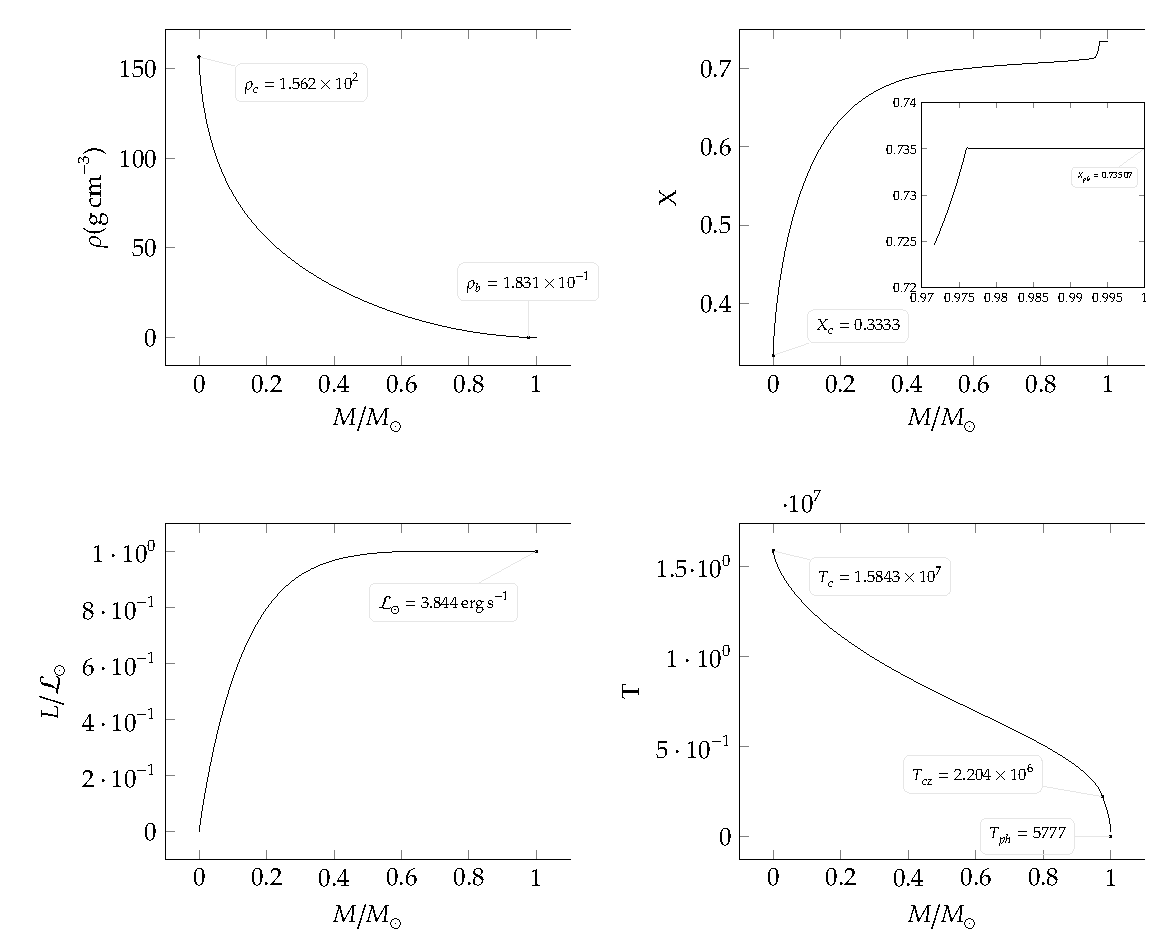
\includegraphics[width=\textwidth,trim=4 4 4 4,clip]{bahcall95}};
}{(0,-7)}{\textwidth}{Profilo radiale della densit\'a, composizione, luminosit\'a e temperatura. Dati da \cite{bahcall95diffusion}.}

%\eqref{eq:massaguscio},\eqref{eq:fidroequilibrio},\eqref{eq:fenergyconservation}, \eqref{eq:ftransportenergy} a partire da $r=0$ produce soluzioni dipendenti da $(P_c,T_c)$, mentre le condizioni alla superficie sono pi\'u complesse perch\'e dipendono dalla struttura dell'atmosfera e le soluzioni sono dipendenti da $(R,L)$: i quattro parametri matematici del problema, $(P_c,T_C,L,R)$, sono determinati dalla condizione di continuit\'a ad un punto intermedio  delle soluzioni $(P,T,m(r),l(r))$ fra le soluzioni con condizioni al centro e sulla superficie.

\end{document}